% options:
% thesis=B bachelor's thesis
% thesis=M master's thesis
% czech thesis in Czech language
% slovak thesis in Slovak language
% english thesis in English language
% hidelinks remove colour boxes around hyperlinks
% 10pt 11pt 12pt

\documentclass[thesis=M,slovak]{FITthesis}[2013/05/06]

\usepackage[utf8]{inputenc} % LaTeX source encoded as UTF-8

\usepackage{graphicx} %graphics files inclusion
\usepackage{hyperref} %hypertext
\usepackage{float}
\usepackage{listings}
\usepackage{tabularx}
\lstset{language=Python,
breakatwhitespace=false,         % sets if automatic breaks should only happen at whitespace
  breaklines=true,                 % sets automatic line breaking
} 
% \usepackage{amsmath} %advanced maths
% \usepackage{amssymb} %additional math symbols

\usepackage{dirtree} %directory tree visualisation

% % list of acronyms
% \usepackage[acronym,nonumberlist,toc,numberedsection=autolabel]{glossaries}
% \iflanguage{czech}{\renewcommand*{\acronymname}{Seznam pou{\v z}it{\' y}ch zkratek}}{}
% \makeglossaries

\newcommand{\tg}{\mathop{\mathrm{tg}}} %cesky tangens
\newcommand{\cotg}{\mathop{\mathrm{cotg}}} %cesky cotangens

\interfootnotelinepenalty=10000

% % % % % % % % % % % % % % % % % % % % % % % % % % % % % % 
% ODTIALTO DALEJ VSETKO ZMENTE
% % % % % % % % % % % % % % % % % % % % % % % % % % % % % % 

\department{Katedra softwarového inženýrství}
\title{Spracovanie a vizualizácia chemických meraní v dátovom repozitári}
\authorGN{Lukáš} %(krstné) meno (mená) autora
\authorFN{Koštenský} % priezvisko autora
\authorWithDegrees{Bc. Lukáš Koštenský} %meno autora včetne súčasných akademických titulov
\supervisor{RNDr. David Antoš, Ph.D.}
\acknowledgements{Rád by som poďakoval RNDr. Davidovi Antošovi, Ph.D. za cenné rady pri písaní práce. Taktiež by som rád poďakoval Mgr. Miroslavovi Šimkovi za pomoc a rady pri návrhu a programovaní aplikácie. Tiež by som chcel poďakovať Ing. Janovi Horníčkovi za pomoc pri získavaní testovacích dát, ich vysvetleniu a vytvorenie testovacích a produkčných serverov pre repozitár.}
\abstractCS{Cieľom diplomovej práce je vytvoriť software, ktorý bude slúžiť ako repozitár vedeckých dát. Zameriava sa pritom na dáta Ústavu organickej chémie VŠCHT Praha. Výsledný repozitár používa rôzne nástroje. Ako jadro repozitára je použitá Fedora, ktorá sa stará o ukladanie dát. Vyhľadávanie rieši Elasticsearch. Bolo vytvorené webové užívateľské rozhranie v programovacom jazyku Python s využitím frameworku Django. Vytvorené boli tiež nástroje pre správu a kontrolu oprávnení a nástroj na import dát z aplikácie Open Enventory.}
\abstractEN{The aim of the diploma thesis is to create software, which will be used as science data repository. It is focused on data from Department of organic chemistry UCT Prague. Final repository uses different tools. Fedora is used as core of repository and takes care about data storing. Elasticsearch is used for searching in repository. Web user interface is created in Python with usage of framework Django. I created also tools for checking and controlling permissions and tool for importing data from Open Enventory.}
\placeForDeclarationOfAuthenticity{V~Prahe}
\declarationOfAuthenticityOption{1} %voľba Prehlásenia (číslo 1-6)
\keywordsCS{Fedora, repozitár, Elasticsearch, webová aplikácia, Python, Django, Java}
\keywordsEN{Fedora, repository, Elasticsearch, web application, Python, Django, Java}
% \website{http://site.example/thesis} %volitelná URL práce, objeví se v tiráži

\begin{document}

% \newacronym{CVUT}{{\v C}VUT}{{\v C}esk{\' e} vysok{\' e} u{\v c}en{\' i} technick{\' e} v Praze}
% \newacronym{FIT}{FIT}{Fakulta informa{\v c}n{\' i}ch technologi{\' i}}

\begin{introduction}
Nielen výskumníci, ale aj bežný užívatelia počítačov riešia problém s ukladaním dát. Tých máme stále viac, musíme ich niekam ukladať a ideálne aj zabezpečiť, že sa nestratia napríklad pri poškodení disku. Výskumníci, na rozdiel od bežných užívateľov, potrebujú závery výskumov, ale aj samotné dáta z meraní publikovať. Aby takto zverejnené množstvo dát bolo pre ostatných použiteľné, musí v nich byť možné vyhľadávať.

Ako centrálne úložisko dát sa bežne používajú repozitáre, takúto službu poskytujú najmä knižnice, školy, ale aj iné inštitúcie. Pre ukladanie a správu ale aj zverejnenie kníh, článkov a iných textových dokumentov existuje niekoľko rôznych softwarov. Dáta uložené v nich sú popisované metadátami.

Existujú štandardizované metadátové schémy, ktoré sú určené na popis metadát ku knihám, článkom ale aj iným dátam. Nie vždy, najmä ak potrebujeme pracovať s dátami z rôznych vedeckých odvetví, je možné existujúcimi metadátovými schémami dostatočne popísať dokumenty.

V prípade vedeckých dát už taktiež nestačí v repozitári zobraziť metadáta a umožniť stiahnuť textový dokument. Rôzne typy dát je potrebné zobraziť rôznymi spôsobmi, v niektorých je taktiež potrebné vyhľadávať, pričom pre vyhľadávanie v nich nemusí stačiť textové zadanie hľadaného výrazu.

Repozitár, ktorý by bol vhodný pre rôzne vedecké dáta, musí vedieť uložiť veľké množstvo dát, v nich vedieť vyhľadávať a tiež ich zobraziť. CESNET, z.s.p.o. má k dispozícii dátové úložisko \cite{DataCare}, nad ktorým je možné vytvoriť repozitár. V rámci diplomovej práce sa teda pokusím vytvoriť software, ktorý bude slúžiť pre ukladanie vedeckých dát. Zamerám sa pritom na dáta Ústavu organickej chémie VŠCHT Praha. Pri vytváraní repozitára využijem, upravím alebo vytvorím vhodné nástroje, ktoré umožnia prácu s dátami.
\end{introduction}

\chapter{Popis problému}
Repozitár slúži vo všeobecnosti ako centrálne miesto, ktoré sa stará o ukladanie a správu dát. Takúto službu môžu chcieť poskytovať rôzne inštitúcie, napríklad školy, knižnice,... Pod slovom repozitár si môžeme taktiež predstaviť konkrétny software, ktorý sa stará o ukladanie, archiváciu a sprístupnenie dát. V tejto diplomovej práci budeme pod slovom repozitár rozumieť práve software.

\section{Zdieľanie dát v tíme}
Ústav organickej chémie VŠCHT Praha potrebuje vyriešiť ukladanie a sprístupnenie dát. Potrebuje ukladať, analyzovať a prezentovať infračervené vibračné, NMR a hmotnostné spektroskopické merania, chemické vzorce a reakcie.

Nad jedným datasetom môže pracovať viacero ľudí, ktorí môžu riešiť rôzne merania a pokusy alebo spoločne pracovať na jednom meraní. V oboch prípadoch počas priebehu samotného výskumu potrebujú prístup k dátam, ktoré vytvoril iný člen tímu. Taktiež musia mať možnosť dáta upravovať (napr. opakované merania a pokusy, keď je potrebné doplniť nové výsledky). Repozitár teda musí umožniť zdieľanie dát v tíme, rôzne oprávnenia pre osoby, ktoré majú mať k dátam prístup, verziovanie dát.

\section{Open data/Open access}
Pri vývoji repozitára je potrebné myslieť na možnosť zverejnenia (časti) dát pre širokú verejnosť s možnosťou ich ďalšieho využitia alebo odkazovania na ne. Takto zverejnené dáta označujeme pojmom Open data. V prípade zverejnených výskumov hovoríme o Open access (OA). Repozitár musí umožniť zverejnenie všetkých alebo časti uložených dát. Cieľom vývoja repozitára je vytvorenie platformy, s využitím ktorej bude možné publikovať nielen články a závery výskumu, ale aj čiastkové merania a experimenty, ktoré k výsledkom viedli.

\section{Zálohovanie a archivácia}
Zálohovaním dát rozumieme vytváranie kópie práve spracúvaných alebo v relatívne nedávnej dobe uložených dát. Archiváciou rozumieme uchovávanie dokumentačných materiálov.

Zálohované dáta môžu byť poškodené degradáciou média, fyzickým poškodením média alebo v súčasnosti rozšírenými cryptovírusmi. Zálohovať dáta na jedno médium nestačí. Je dobré sa riadiť pravidlom 3-2-1. Tri kópie všetkých dôležitých dát, na dvoch rôznych médiách, pričom jedna kópia by mala byť uložená off-site, teda niekde mimo pracovného prostredia. \cite{zalohovanie}

Pri archivácii dát je potrebné myslieť na čitateľnosť dát po dlhej dobe. Preto je potrebné myslieť nielen na zabezpečenie dát, ale aj na archiváciu programu potrebného na prečítanie archivovaných dát.

Repozitár by mal byť pre užívateľov možnosťou ako dáta zálohovať. Zároveň jeho napojenie na služby CESNETu umožní ochranu dát, akú by bolo na pracovisku VŠCHT Praha ťažké dosiahnuť.

V budúcnosti bude možné repozitár rozšíriť o nástroje, ktoré by umožnili aj dlhodobú archiváciu dát.

\chapter{Súčasné riešenia}
\section{Repozitáre}
Existujú rôzne repozitáre, ktoré sa od seba líšia použitou technológiou, možnosťou rozšírenia, používajú rôzne metadátové schémy. Niektoré sú voľne dostupné ako open source, iné ako proprietárny software alebo hosťované aplikácie. V tejto časti uvádzam prehľad dostupných aplikácií. Zameriavam sa najmä na vlastnosti, ktoré boli pre ďalší vývoj repozitára kľúčové, a to: open source (aby bolo možné software ďalej upravovať), použitie metadátovej schémy, modulárnosť softwaru (jednoduchá možnosť rozšírenia o ďalšie nástroje) a verziovanie (najmä kvôli zdieľaniu a zálohovaniu dát).

% Tento software sa zameriava na dokumenty, ktoré majú byť voľne dostupné (anglicky Open Access) a online. Najčastejšie sa do takýchto inštitucionálnych repozitárov ukladajú textové dokumenty, pre ktoré je software najlepšie prispôsobený.

\subsection{Metadáta}
Na popis uložených dokumentov slúžia metadáta. Metadáta sú štrukturované dáta nesúce informáciu o primárnych dátach. Pojem metadát je používaný predovšetkým v súvislosti s elektronickými zdrojmi. \cite{iso8459-5} Za zdroje alebo dokumenty pokladáme knihy, články, časopisy, audio nahrávky, obrazové záznamy, binárne súbory obsahujúce dáta z meraní a ďalšie. Kvôli vzájomnej prepojenosti repozitárov, vyhľadávaniu dát a správnej interpretácii informácií je snaha o~vyvinutie celosvetovo používaného štandardu pre popis dát. 

O to sa snažia rôzne metadátove schémy, pomocou ktorých je možné zdroje popísať. Medzi najznámejšie schémy patrí Dublin Core [\url{http://dublincore.org/}] a MARC [\url{http://www.loc.gov/marc/}].

\subsubsection{Dublin Core}
Dublin Core (skrátene DC) vznikol s cieľom jednoducho a všeobecne popísať zdroje. Metadátová schéma je určená pre popis zdrojov umiestnených na web. Táto schéma obsahuje 15 prvkov. To sú: názov (title), autor (creator), predmet (subject), popis (description), vydavateľ (publisher), prispievateľ (contributor), dátum (date), typ (type), formát (format), identifikátor (identifier), zdroj (source), jazyk (language), vzťah (relation), pokrytie (coverage) a práva (rights). \cite[s.~37]{zhang2014creating} Tieto prvky nie sú povinné a môžu sa opakovať. Jednotlivé vlastnosti sú teda pomenované. Ako sa World Wide Web menil, v snahe o vytvorenie sémantického webu vyvinul sa aj štandard Dublin Core. Od roku 2008 obsahuje formálne domény a rozsahy v definíciách vlastností. Tento aktualizovaný variant vlastností sa nazýva dcterms. Jednotlivé prvky môžu byť ďalej rozšírené o kvalifikátor. Ten môže lepšie určiť, čo daná položka popisuje. Napríklad namiesto všeobecného autora tak môžeme upresniť, či išlo o ilustrátora (dc:creator.ilustrator), editora (dc:creator.editor),...  Kvalifikátory ale nesmú meniť význam vlastnosti, dokument popísaný s využitím kvantifikátorov tak ostáva kompatibilný aj pre systémy, ktoré kvantifikátory nepoužívajú.\cite[s.~295]{witten2009build}

\subsubsection{MARC}
MARC (MAchine-Readable Cataloging) využívajú najmä knihovníci. Bol navrhnutý pre popis bibliografických údajov v strojovo čitateľnej podobe.
Schéma obsahuje vlastnosti, ktoré sú očíslované. Kým názov v dcterms je označený ako title, v MARCu  je označený číslom 245 (title proper statement). Na rozdiel od dcterms obsahuje niekoľko pomocných polí (ako napríklad 222 kľúčový názov, 240 unifikovaný názov,...).\cite[s.~288-289]{witten2009build} Takéto označenie je ľahko čitateľné pre stroje, knihovníci si pri každodennej práci s týmito číslami ich významy zapamätajú. Človek, ktorý ich vidí prvýkrát, významu nerozumie.

MARC je od DC komplikovanejší, dokáže však presnejšie popísať zdroj.
Prvé číslo v číselných kódoch určuje, o aký typ informácie ide, jednotlivé kódy sú popísané v tabuľke \ref{tab:marc}. V prípade kódov 1XX, 4XX, 6XX, 7XX a 8XX sa obsah upresňuje doplnením dvojice čísel. Zvyčajne sa dodržiavajú nasledujúce dvojice: X00 - Mená osôb, X40 - Bibliografické názvy, X10 - Názvy firiem, X50 - Tematické pojmy, X11 - Názvy stretnutí/konferencií, X51 - Názvy miest, X30 - Jednotné názvy.

\begin{table}[!htbp]\centering
 	\caption[MARC]{Typ informácie v kóde MARC}\label{tab:marc}
\begin{tabularx}{\textwidth}{|l|X|} \hline
0XX	& Kontrolná informácia, identifikačné a klasifikačné čísla,... \\ \hline
1XX	& Hlavné údaje \\ \hline
2XX	& Názvy a kapitoly (názov, edícia, vydanie) \\ \hline
3XX	& Fyzický popis,... \\ \hline
4XX	& Informácie o dieloch/sériách \\ \hline
5XX	& Poznámky \\ \hline
6XX	& Kontaktné informácie na subjekty \\ \hline
7XX	& Pridané informácie (iné než o subjektoch, dieloch/sériách); linkovacie polia \\ \hline
8XX	& Rada pridaných informácií, informácie o holdingoch \\ \hline
9XX	& Vyhradené pre lokálnu implementáciu \\ \hline
\end{tabularx}
\end{table}

Hodnoty niektorých kódov majú presne určenú dĺžku a obsah, napríklad kód 008 obsahuje číselný kód pre zdroj a kód jazyka, v akom je dokument napísaný. Iné polia nemajú obmedzenú dĺžku ani definovanú štruktúru a hodnoty v nich sú len textové polia. Tieto polia často obsahujú aj podhodnoty, ktoré sú označené písmenami a, b, c,.... Napríklad pole s kódom 100 (meno autora) môže obsahovať podpolia so štandardizovaným menom, celými krstnými menami a dátumi.\cite[s.~288-291]{witten2009build}

Použitie navrhovaného repozitára by malo byť jednoduché aj pre užívateľov, ktorí s metadátami nemajú veľké skúsenosti a nepotrebujú komplikovaný popis dát. Pre skúsenejších užívateľov by však bolo dobré zachovať možnosť použitia zložitejších, prípadne vlastných metadátových schém. Repozitár by teda mal vedieť používať aj iné metadátove schémy než len Dublin Core alebo MARC.

\subsection{Software}
V tejto časti popisujem prehľad najrozšírenejších softwarov, ktoré sa používajú ako implementácie repozitárov. Uvádzam prehľad dôležitých vlastností pre ďalší vývoj repozitára a to, či ide o proprietárny alebo open source systém, kvôli možnosti ďalších úprav; programovací jazyk a modulárnosť softwaru; aké metadátové schémy používajú a či ich je možné rozširovať; a či daný software umožňuje verziovanie uložených dát.

Keďže každý software pokrýva inú kombináciu týchto vlastností, bolo by veľmi náročné pokúšať sa o nejakú klasifikáciu. Preto uvádzam len prehľad ich vlastností:

\subsubsection {Digital Commons}  [\url{http://digitalcommons.bepress.com/}]

Hostovaná platforma inštitucionálneho repozitára. Zameraný na školy a školské dokumenty.

Používa Dublin Core schému, v používateľskom rozhraní podporuje aj iné vlastnosti než len DC, aj keď nepodporuje iné schémy (vrátane MARC).

Autori vedia prispôsobiť repozitár požiadavkám klienta.

Nepodporuje verziovanie.

\subsubsection {LIBSYS}  [\url{http://www.libsys.co.in/}]

Proprietárny software. Repozitár funguje ako webová aplikácia.

Používa MARC ako schému metadát.

\subsubsection {SimpleDL}  [\url{http://www.simpledl.com/}]

Proprietárny software.

Metadáta na základe Dublin Core. Môžu byť rozšírené o iné schémy.

\subsubsection {Greenstone}  [\url{http://www.greenstone.org/}]

Repozitár vyvinutý na Univerzite Waikato.

Používa MARC schému.

Modulárna architektúra, napísaný v jazyku Java. Pluginy v jazyku Perl.

Nepodporuje verziovanie.

Open source

\subsubsection {Invenio}  [\url{http://inveniosoftware.org/}]

Software bol pôvodne vyvinutý pre CERN. Umožňuje vytvoriť digitálnu knižnicu alebo repozitár dokumentov dostupný cez web. 

Používa špecifikáciu MARC pre metadáta.

Má modulárnu architektúru. Napísaný v jazyku Python.

Podporuje verziovanie uložených dát.

Open Source

%\subsubsection {Zenodo} [\url{https://zenodo.org/}]
%
%Vyvinutý na základe Invenia, taktiež pre CERN. Má teda rovnaké vlastnosti ako Invenio.

\subsubsection {EPrints} [\url{http://www.eprints.org/}]

Vyvinutý na Univerzite Southampton.

Používa rôzne typy metadátových polí, ktoré je možné nastavovať (upraviť zobrazovanie, indexovanie, vyhľadávanie).

Modulárny software napísaný v jazyku Perl.

Podporuje verziovanie dát.

Open Source

\subsubsection {DSpace} [\url{http://www.dspace.org/}]

Software pôvodne vyvinutý MIT a Hewlett-Packard. Od vzniku má viac ako 2000 inštalácií po celom svete. 

Ako východziu schému pre popis dát používa Dublin Core, je však možné použiť aj iné schémy.

Ide o súbor spolupracujúcich Java webových aplikácií. K dispozícii je RESTful webové užívateľské rozhranie.

Neumožňuje verziovanie uložených dát.

Open source

\subsubsection {Fedora} [\url{http://www.fedora-commons.org/}]

Je možné použiť rôzne schémy pre popis dát.

Flexibilný, jednoducho rozšíriteľný, modulárny repozitár. Napísaný v programovacom jazyku Java.

Umožňuje verziovanie uložených dát.

Open Source


\section{Nástroje na zber a organizáciu chemických dát}
Výskumníci v oblasti chémie si vedú laboratórne denníky so záznamami hypotéz, experimentov, analýz alebo interpretáciou experimentov. V súčasnosti sa denníky vedú v elektronickej forme s využitím elektronických laboratórnych denníkov (často sa pre tento software používa skratka ELN). Keďže Ústav organickej chémie VŠCHT Praha používa a naďalej chce používať len E-Notebook a Open Enventory, iné nástroje na zber a organizáciu chemických dát v prehľade neuvádzam.

Prehľad programov, ktoré používa Ústav organickej chémie VŠCHT Praha:
\subsection{E-Notebook} [\url{http://www.cambridgesoft.com/Ensemble/E-notebook/}]
Software od firmy Perkin Elmer. V súčasnosti je k dispozícii len ako Enterprise verzia alebo ako súčasť cloudových aplikácií Elements \url{https://elements.perkinelmer.com/} a plánovaného ChemDraw E-notebook \url{http://chemdrawenotebook.perkinelmer.cloud/}. Perkin Elmer dodáva Enterprise aplikáciu ako hotové riešenie s úpravami a nastavením pre konkrétného zákazníka. Software funguje na serveroch Oracle. Cloudové riešenie aj Enterprise verzia softwaru je uzatvorená a upravovať ich môže len dodávateľská firma.

\subsection{Open Enventory} [\url{https://www.chemie.uni-kl.de/goossen/open-enventory/}]
Webová open source aplikácia napísaná v jazyku PHP, ktorá má k dispozícii všetky zdrojové kódy. Neexistuje k nej ale žiadna dokumentácia. 
Pri prechádzaní kódu aplikácie som naviac zistil, že veľká časť komentárov a aj časť samotného kódu sú napísané v nemčine. 

Využíva MySQL databázu. Databázová schéma taktiež nie je prehľadná, v jednotlivých tabuľkách nie sú označené cudzie kľúče, a teda chýbajú prepojenia na iné tabuľky. Na stĺpcoch, ktoré by mali byť cudzími kľúčmi, sú len indexy.

\chapter{Analýza a návrh riešenia}
\section{Analýza požiadaviek}
CESNET, z.s.p.o. bol oslovený Ústavom organickej chémie VŠCHT Praha, ktorý potrebuje vyriešiť ukladanie a sprístupnenie vlastných dát - chemické vzorce, reakcie, analýzi nameraných dát. Nad jedným datasetom môže pracovať viacero výskumníkov, niektorí dáta namerali, iní ich analyzujú alebo každý člen tímu pracujúci na jednom projekte rieši iné merania a experimenty. Výskumník teda okrem vlastných dát potrebuje mať prístup aj k dátam ostatných ľudí v tíme. Nie všetky dáta môžu byť zverejnené, na niektoré výskumy môže platiť embargo a majú byť zverejnené až neskôr, k dátam, s ktorými sa aktuálne pracuje majú mať prístup len členovia teamu alebo dáta ich autor nechce zverejniť z iných dôvodov. Pre tieto dáta taktiež potrebujú vyriešiť zálohovanie.

Ako sa postupne zistilo, o vyriešenie ukladania a sprístupnenia dát má záujem viacero rôznych a na rôzne dáta zameraných skupín. Preto chceme vytvoriť repozitár, ktorý bude jednoduché rozšíriť pre užívateľov používajúcich iné typy dát a metadát.

CESNET v rámci služieb DataCare poskytuje dátové úložisko s celkovou hrubou kapacitou presahujúcou 21 PB. Toto úložisko poskytuje dátovy priestor pre zálohovanie, archiváciu, zdielanie dát. \cite{DataCare} Úložisko dát umožňuje ukladať dáta tak, aby boli prístupné len pre jednu osobu alebo zdielané pre skupinu ľudí. Služba FileSender umožňuje rychlé a jednoduché odosielanie veľkých súborov až stovkám prijímateľov, OwnCloud umožňuje sprístupniť dáta cez webové rozhranie a synchronizovať ich s inými zariadeniami alebo zdielať s inými ľuďmi. \cite {DatoveUloziste} CESNET teda má vytvorené zázemie, ktoré bude možné využiť pre potreby repozitára.

\subsection{Funkčné požiadavky}

Ústav organickej chémie VŠCHT Praha v súčasnosti využíva aplikácie pre tvorbu laboratórnych denníkov, v ktorých sú uložené informácie o chemických prvkoch, reakciách, ktoré počas pokusu nastali. Taktiež priebeh meraní a pokusov. Aby bola využiteľnosť repozitára čo najlepšia a práca s ním čo najjednoduchšia, požadujú možnosť importovať dáta z aplikácie Open Enventory, v ktorej si vedú laboratórne denníky, do repozitára. 

Projekty v rámci laboratórnych denníkov obsahujú: 
		\begin{itemize}
			\item meno vedca alebo vedcov, ktorí na meraniach a pokusoch spolupracovali,
			\item priebeh meraní a pokusov,
			\item reaktanty,
			\item vzniknuté produkty,
			\item chemickú rovnicu, ktorá bude zobrazená aj schematicky (obrázkom),
			\item pozorovanie priebehu pokusu,
			\item NMR spektrá (spektrá nukleárnej magnetickej rezonancie) chemických prvkov,
			\item IR (infračervené) spektrá,
			\item hmotnostné spektrá,
			\item pri chemických prvkoch je potrebné evidovať:
				\begin{itemize}
					\item štandardný názov prvku,
					\item zápis štruktúry,
					\item obrázok štruktúry,
					\item chemický vzorec prvku,
					\item molekulárnu hmotnosť,
					\item hmotnosť prvku,
					\item koncentráciu.
				\end{itemize}
		\end{itemize}

Repozitár musí pre tieto dáta umožniť:
\begin{itemize}
	\item Uložiť nové dáta.
	\item Upraviť existujúce dáta.
	\item Zobraziť existujúce dáta.
	\item Uložiť históriu zmien dát.
	\item Vyhľadávanie v metadátach.
	\item Kontrolovať oprávnenia na prístup k dátam.
	\item Import dát z aplikácie Open Eventory.
\end{itemize}

Prístup k jednotlivým dokumentom a poliam ale môže byť limitovaný. Vytváranie a úprava jednotlivých dokumentov je umožnená len konkrétnym užívateľom.

Aplikácia Open Eventory musí byť upravená tak, aby umožnila export dát vo formáte vhodnom pre import do repozitára.

\subsection{Požiadavky na vlastnosti repozitára}
\begin{itemize}
	\item Repozitár bude pre užívateľov dostupný ako webová aplikácia.
	\item Repozitár musí umožniť ďalšie rozšírenie pre iné typy dát.
	\item Repozitár bude napojený na služby CESNETu.
\end{itemize}

\subsection{Administračné rozhranie}
Aby bolo možné spravovať kolekcie, oprávnenia pre prístup, užívateľov priamo v aplikácii, je potrebné vytvoriť v repozitári administračné rozhranie. Implementácia tohto rozhrania ale nie je súčasťou tejto diplomovej práce.

Z požiadaviek na umožňenie rozšírenia pre ďalšie typy dát plynie nutnosť vytvoriť nástroje, ktoré umožnia vytvoriť a spravovať šablóny pre zobrazenie, vytvorenie a editáciu týchto dát. Môžeme predpokladať, že tieto šablóny síce bude vytvárať osoba, ktorá má aspoň nejaké skúsenosti s tvorbou HTML šablón, nedá sa predpokladať skúsenosť s programovaním v Pythone a frameworku Django. 

Administračné rozhranie by teda malo poskytovať aj nástroje pre tvorbu a úpravu HTML šablón pre jednotlivé typy dokumentov. Taktiež tvorbu modelov pre jednotlivé typy dokumentov.
Rozhranie pre vytváranie a editáciu oprávnení pre jednotlivé kolekcie, dáta alebo metadátové polia, správu užívateľov a skupín.


\section{Výber technológií}
\subsection{Výber repozitára}
Keďže ani jeden existujúci repozitár nespĺňa všetky požiadavky alebo nevie uložiť/zobraziť dáta pre Ústav organickej chémie VŠCHT Praha, bolo potrebné vytvoriť nový alebo upraviť stávajúci software. Vytvorenie nového softwaru od základov by bolo neefektívne. Vyššie zmienené repozitáre fungujú, niektoré ich časti by teda boli programované nanovo. Zvolená bola možnosť doplniť/upraviť funkčnosť existujúceho repozitára. Keďže zadávateľ preferuje open source riešenia, výberali sme vhodný repozitár z open source repozitárov.

Okrem toho boli pri výbere vhodného repozitára do úvahy brané ďalšie kritériá. A to možnosť použitia viacerých metadátových schém, programovací jazyk, podpora komunity. Do finálneho výberu sa dostali DSpace a Fedora. Z testov, ktoré sme pri výbere repozitára previedli, vyplynulo, že sú oba repozitáre podobne výkonné. Vyhľadávanie v metadátach bude naviac zabezpečené samostatnou aplikáciou. Oba zvládajú milióny záznamov \cite{Fedora} \cite[s.~213]{DigitalLibrary}.

Vďaka návrhu Fedory je pridávanie rozšírení do tohto softwaru jednoduchšie, taktiež už má vyriešené verziovanie uložených dát. DSpace má k dispozícii webové užívateľské rozhranie, ktoré je možné upravovať a ďalej rozširovať. Fedora používa jednoduché webové rozhranie, ktoré umožňuje len základnú prácu s dátami. Vytvorenie samostatného, nového webového užívateľského rozhrania s využitím RESTapi je ale jednoduchšie než úprava jadra DSpace, aby zvládal verziovanie uložených dát.

Z existujúcich možností bola zvolená Fedora ako najvhodnejší software pre možnosť ďalších potrebných úprav pre použitie v rámci služieb CESNET z.s.p.o. a splnenie požiadaviek Ústavu organickej chémie VŠCHT Praha.

Základné webové rozhranie, ktoré poskytuje Fedora umožňuje zobraziť metadáta, stiahnuť binárne súbory, vytvoriť potomka typu kontajner a binárny dokument, upraviť alebo zmazať existujúci dokument. Za kontajner sú vo Fedore považované všetky dokumenty okrem binárnych, teda aj tie, ktoré už žiadneho potomka nemajú. Binárneho typu sú dokumenty obsahujúce dátové súbory nahrané do Fedory. Webové rozhranie je možné vidieť na obrázku \ref{graphics:fedora}.

Pre účely repozitára dát pre Ústav organickej chémie VŠCHT Praha je takéto zobrazenie dát nedostatočné. Bolo potrebné vytvoriť užívateľské rozhranie, ktoré vhodným spôsobom zobrazí zoznam dokumentov vrámci kolekcie ale aj samotné dáta a metadáta dokumentu.

Vytvorené webové užívateľské rozhranie tiež musí umožniť vyhľadávanie v uložených dátach.

Existujúce rozhranie umožňuje vytvoriť nový dokument a následne k nemu pridať informácie. Tie je možné zadávať len v textovej forme s využitím jazyka RDF (Resource Description Framework), teda trojíc - subjekt, predikát a objekt. RDF je jazyk používaný pre reprezentáciu informácii na webe. \cite{RDF} Preto je potrebné zjednodušiť vytváranie nových kolekcií a dokumentov v užívateľsky prívetivej forme.

Pre vytváranie nových dokumentov, úpravu existujúcich a zobrazenie dát bude potrebné vytvárať HTML šablóny. Repozitár má byť čo najľahšie rozšíriteľný pre rôzne dáta a metadáta. Preto bolo potrebné vytvoriť nástroj, ktorý umožnil používanie šablón pre nove typy dát s čo najmenším zásahom do kódu aplikácie. Tento nástroj vie pracovať so šablónami uloženými priamo vo Fedore.

Prístupové práva je taktiež možné nastaviť pomocou RDF priamo v existujúcom webovom rozhraní. Musím však prácu s nastavovaním a kontrolou oprávnení zjednodušiť. Na to bolo potrebné upraviť aj kód Fedory.

\begin{figure}\centering
	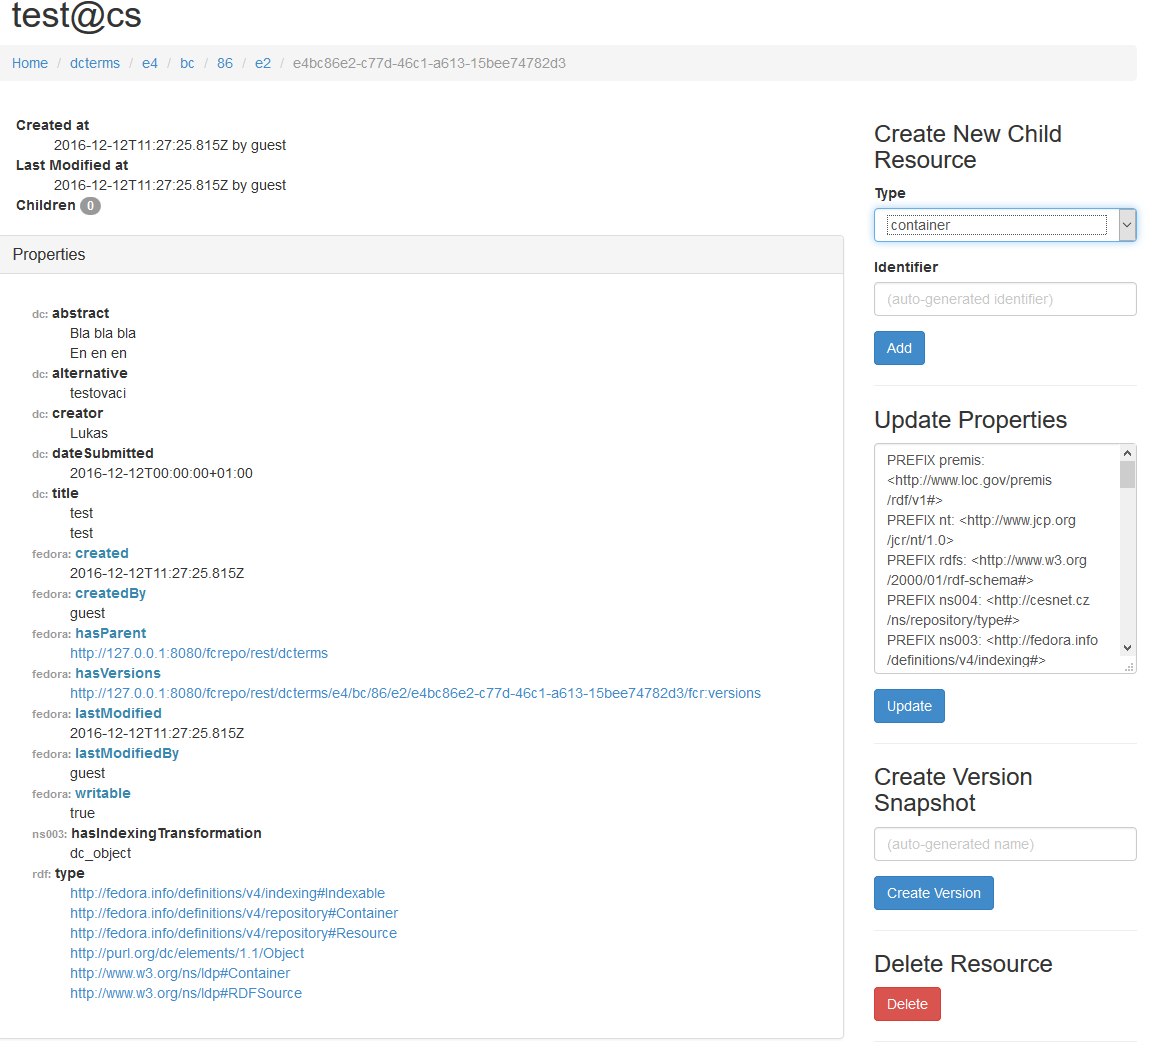
\includegraphics[width=1.0\textwidth]{fedora/dcterms_vo_Fedore.png}
 	\caption[Zobrazenie dát vo webovom rozhraní Fedory]{Zobrazenie dát vo webovom rozhraní Fedory}\label{graphics:fedora}
\end{figure}

\subsection{Výber aplikácie pre vyhľadávanie}
Na vyhľadávanie v repozitári bude použitá samostatná aplikácia. Synchronizáciu dát s Fedorou zabezpečuje medzivrstva, ktorá komunikuje s oboma aplikáciami. Potrebujeme teda aplikáciu na vyhľadávanie v textových metadátach, ktorá je čo najrýchlejšia a zvláda veľké množstvo (milióny) záznamov.

Keďže zadávateľ preferuje open source, pri výbere sme sa rozhodovali medzi týmito najrozšírenejšími vyhľadávacími aplikáciami:
\subsubsection{ElasticSearch \url{https://www.elastic.co/products/elasticsearch}}

ElasticSearch je distribuovaný, RESTful vyhľadávaci a analytický software. Umožňuje veľmi rýchle vyhľadávanie v indexovaných dátach. Dopyty je možné posielať s využitím RESTful api a JSONu, knižnice sú dostupné pre rôzne programovacie jazyky vrátane Pythnu a Javy. Podľa \cite{NajpouzivanejsieVyhladavace} ide o najrozšírinejší vyhľadávaci engine.

\subsubsection{Solr \url{http://lucene.apache.org/solr/}}

Solr je taktiež RESTful vyhľadávací software s podporou pre dáta vo formáte JSON, XML, CSV alebo binárnych dát cez HTTP.

Obe vyhľadávacie aplikácie vychádzajú z jadra Apache Lucene, čo je vysokovýkonná, plnohodnotná, v texte vyhľadávacia knižnica napísaná v Jave. Umožňuje full-textové vyhľadávanie v dokumentoch. \url{http://lucene.apache.org/core/}

\subsubsection{Porovnanie vyhľadávacích aplikácií}
V tabuľke \ref{tab:searchEngines} je porovnanie vlastností, ktoré rozhodovali pri výbere vyhľadávacieho enginu.

\begin{table}[!htbp]\centering
 	\caption[ElasticSearch vs. Solr]{Porovnanie vyhľadávacích enginov}\label{tab:searchEngines}
\begin{tabularx}{\textwidth}{|l|X|X|} \hline
Vlastnosť & Solr                         & ElasticSearch \\ \hline
Formát vstupných dát   & XML, CSV, JSON	 & JSON \\ \hline
HTTP REST API & Áno & Áno \\ \hline
Knižnice pre Javu & Áno & Áno \\ \hline
Knižnice pre Python & Áno, vytvorená komunitou & Áno \\ \hline
Integrácia vo frameworku Django & Áno & Áno \\ \hline
Vnorené dokumenty & Nie & Áno \\ \hline
Vzťah rodič-potomok & Nie & Áno \\ \hline
\end{tabularx}
\end{table}

Vnorené dokumenty a možnosť vyhľadávať rodičov, ktorých deti spĺňajú špecifikovanú podmienku a opačne vyhľadávať potomkov, ktorých rodičia spĺňajú špecifikovanú podmienku viedli k tomu, že je v repozitári použitý ElasticSearch ako vyhľadávací software. Medzivrstva ale umožňuje pracovať aj s aplikáciou Solr.

\subsection{Výber programovacieho jazyka a frameworku pre vytvorenie užívateľského rozhrania}
Na vývoji repozitára pracuje viacero ľudí, každý ovláda a preferuje iné jazyky. Keďže sme sa rozhodli využiť Fedoru ako repozitár dát a implementovať vlastné webové rozhranie, bolo potrebné určiť programovací jazyk, v akom má byť toto rozhranie naprogramované.

Fedora je vytvorená s využitím programovacieho jazyka Java, ja som mal okrem Javy skúsenosti s PHP, Pythnom a ďalšími programovacími jazykmi, ktoré sa ale pre tvorbu webových aplikácií zvyčajne nepoužívajú alebo som s nimi mal len minimálne skúsenosti. Mgr. Miroslav Šimek, ktorý vytváral repozitár záverečných prací na VŠCHT Praha má najväčšie skúsenosti s vývojom aplikácií v Pythone s využitím frameworku Django. Väčšina webových služieb, ktoré ma na VŠCHT na starosť oddelenie CIS (Centrum informačných služieb) a práve Mgr. Miroslav Šimek, využíva Python a framework Django.

Zhodnotil som svoje možnosti naučiť sa Django a nakoniec sme sa rozhodli pre využitie Pythonu \url{https://www.python.org/} ako programovacieho jazyka pre vytvorenie webového rozhrania a frameworku Django \url{https://www.djangoproject.com/}, ktorý by mal prácu uľahčiť.

\subsubsection{Python}
Python je interpretovaný programovací jazyk vyššej úrovne. Obsahuje efektívne dátové štruktúry a umožňuje jednoduchý, ale efektívny prístup k objektovo-orientovanému programovaniu. \cite{Python}

\subsubsection{Django}
Django je webový framework pre Python. Na prvý pohľad na fungovanie Djanga sa zdá, že využíva návrhový vzor MVC (Model-view-controller), avšak kontrolérom nazveme v prípade Djanga \uv{view} a view podľa vzoru MVC \uv{template}. V Django interpretácii vzoru MVC ale \uv{view} popisuje dáta, ktoré sú zobrazené užívateľovi. Pritom nie je dôležité ako sa dáta zobrazia, podstatné je, ktoré dáta budú zobrazené.

Obsah dát je oddelený od prezentácie dát. K prezentácii sú využívané šablóny (\uv{template}), ktoré definujú ako sú dáta zobrazené.

Kontrolér podľa definicie MVC je v prípade Djanga skôr framework samotný. Kód, ktorý obslúži dopyt a požiadavok pošle na správné view podľa konfigurácie Django URL. V konfigurácii Django URL sú regulárne výrazy. Ak sa splní niektorý z výrazov, zavolá sa funkcia, ktorá má na starosť obslúženie požiadavkov z danou URL adresou.

Preto sa používa skôr označenie MTV (Model-template-view), ktoré presnejšie popisuje to ako funguje Django. \cite{DjangoFAQ}

Model je klasická dátová vrstva, ktorá obsahuje logiku potrebnú pre prácu s dátami.

\chapter{Implementácia}
\section{Návrh aplikácie}
\begin{figure}\centering
	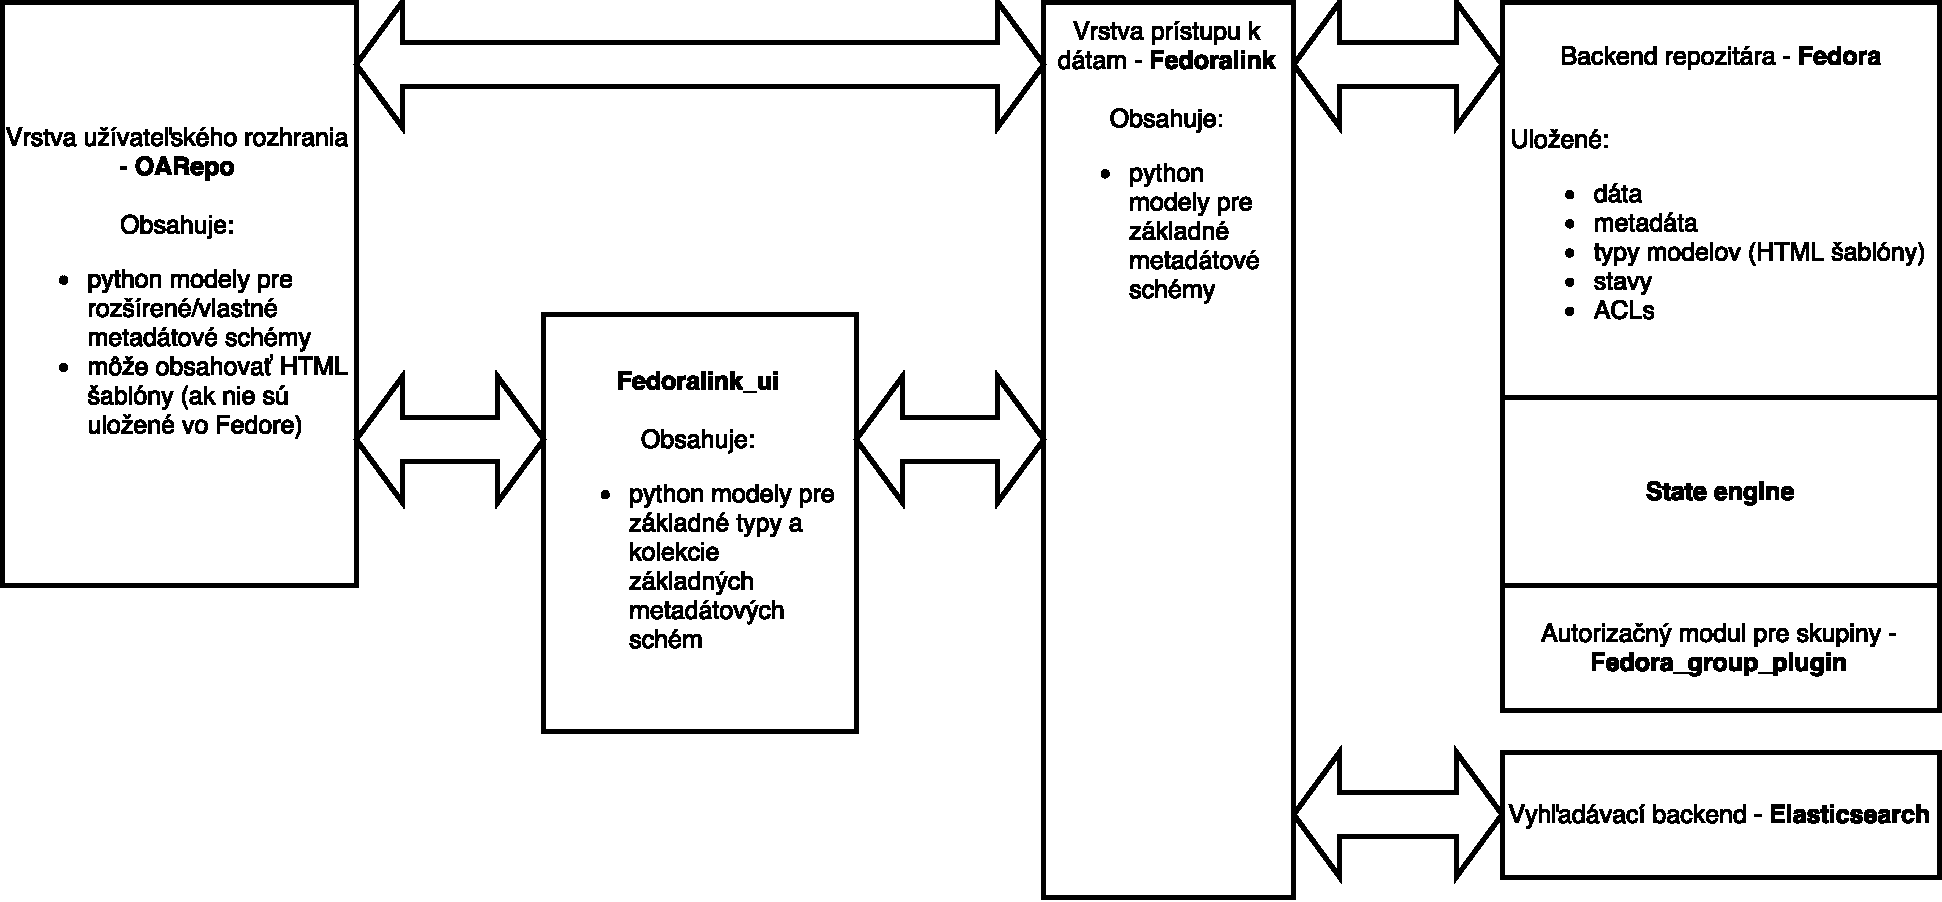
\includegraphics[width=1.0\textwidth]{diagramy/Architektura_repozitara.pdf}
 	\caption[Architektúra repozitára]{Architektúra repozitára}\label{graphics:architektura_repozitara}
\end{figure}


Ako backend repozitára je použitá Fedora. Pre zjednodušenie práce s oprávneniami budú použité stavy. Tento stav je dokument uložený vo Fedore, ktorý môže napríklad vyjadrovať stav publikovania dát (novovytvorený dokument, v procese schvalovania, schválený dokument). Stav obsahuje informáciu o oprávneniach (kto má právo dokument s týmto prideleným stavom vidieť, kto ho môže upravovať,...) a povolené zmeny stavov. Takto je možné dokumentom meniť stavy, v akých sa nachádzajú a meniť tak oprávnenia. Nebude takto potrebné pre každý dokument definovať nové oprávnenia.

Fedora síce umožňuje definiciu prístupových práv (ACLs, z angličtiny Access Control Lists teda zoznamy prístupových práv), ale stavy nepoužíva. Je ju preto potrebné upraviť tak, aby s týmito stavmi vedela pracovať (kontrolovať prechody medzi stavmi). To zabezpečí modul State engine, ktorý upraví kód Fedory.

Oprávnenia chceme nastavovať nielen pre konkrétných užívateľov, ale aj pre rôzne skupiny, do ktorých užívatelia patria. Zároveň sme pri návrhu repozitára mysleli na možnosť prihlásenia cez rôzne autorizačné služby ako je Shibboleth (\url{https://shibboleth.net/}) alebo Perun (\url{https://perun.cesnet.cz}). Využijeme štandardnú On-Behalf-Of HTML hlavičku, s ktorou vie pracovať Fedora a vlastnú On-Behalf-Of-Django-Groups hlavičku. Pre spracovanie tejto hlavičky je nutné do Fedory doplniť autorizačný modul (Fedora\_group\_plugin), ktorý bude súčasťou Fedory.

Užívateľské rozhranie chceme vytvoriť s využitím programovacieho jazyka Python a frameworku Django. Pre možnosť vytvorenia rôznych užívateľských rozhraní pre rôzne používateľské skupiny (ktoré potrebujú pracovať s inými dátami a metadátami) boli vytvorené medzivrstvy Fedoralink a Fedoralink\_ui. Fedoralink má na starosť komunikáciu s Fedorou a Elasticsearchom s využitím REST api. Umožňuje pracovať s dokumentmi získanými z Fedory ako s Django objektmi. Django objekt je inštancia nejakej triedy, s ktorou je možné pracovať podľa definovaných štandardov frameworku Django. Fedoralink dokáže metadáta podľa ich typu získavať z Elasticsearch alebo z Fedory. S využitím Elasticsearch aplikácia taktiež môže v repozitári vyhľadávať.

Fedoralink\_ui je aplikácia napísaná v jazyku Python s využitím frameworku Django, ktorá obsahuje logiku pre prácu so šablónami. Tie chceme ukladať priamo v repozitári, bolo teda potrebné vytvoriť nástroj, ktorý dokáže z repozitára získať správne šablóny, cachovať ich a po doplnení dát z dokumentov do HTML šablóny zobraziť výslednú webovú stránku.

Samotná aplikácia OARepo obsahuje modely a prípadne šablóny, ak nie sú uložené vo Fedore, pre jednotlivé typy dát. Tieto modely definujú vlastné alebo rozširujú existujúce metadátové schémy. Model je trieda v Pythone, po získani dokumentu z Fedory aplikácia vytvorí objekt v Pythone, ktorý je inštanciou takejto triedy (modelu).

Navrhnutú architektúru repozitára je možné vidieť na obrázku \ref{graphics:architektura_repozitara}. Nižšie sú detailnejšie rozpísané funkcie jednotlivých modulov.

\subsection{Fedora}
Ako už bolo zmienené v predchádzajúcej kapitole, ako backend pre repozitár bola zvolená Fedora. V nej sú uložené dáta, metadáta, typy modelov spolu s HTML šablónami, stavy a oprávnenia (ACL).

Metadáta vo Fedore sú uložené s využitím RDF (Resource Description Framework), teda ako trojice - subjekt, predikát a objekt.

\subsection{State engine}
Pre možnosť využívania stavov bude nutné rozšíriť Fedoru o tento modul. Modul rieši prechody medzi stavmi, zmenu stavov, zmenu kontroléru stavov, konkrétnu operáciu povolí len oprávneným osobám. Oprávnené osoby sú určené pomocou ACL. Keďže návrh dátového formátu pre popis stavov pracujúcich s prístupovými právami nadväzujúcimi na štandard W3C WebAccessControl a implementácia tohto modulu boli uvedené ako časť zadania, podrobnejšie sa tomuto modulu venujem v samostatnej sekcii \ref{stavy}.

\subsection{Fedora\_group\_plugin}
Doplňujúci modul do Fedory, ktorý umožňuje overenie oprávnení aj na základe členstva v django skupinách. Framework Django má vyriešenú prácu s užívateľmi, obsahuje kód, ktorý umožňuje ich registráciu, prihlásenie, v administračnom rozhraní správu užívateľov a tiež užívateľských skupín. Pre skupiny je možné nastaviť rôzne oprávnenia. Priamo v kóde aplikácie, využívajúcej framework Django, je tak možné získať objekt, ktorý obsahuje informácie o prihlásenom užívateľovi. Takto sa vieme dostať k jeho používateľskému menu, ale aj ku skupinám, ktorých je členom. 

Samotná Fedora s webac umožňuje overenie autorizácie na základe štandardnej On-Behalf-Of hlavičky, o ktoré sa stará DelegateHeaderPrincipalProvider. On-Behalf-Of HTTP hlavička umožňuje impersonifikáciu na iného užívateľa. Často sa používa, aby administrátor mohol testovať systém ako niektorý z užívateľov alebo simulovať chybu, ktorá niektorému užívateľovi nastala. 

Fedora musí bežať pod Java Servlet kontajnerom (Tomcat, GlassFish, Jetty...), autentizáciu rieši s využitím týchto kontajnerov. Užívateľské údaje sú definované v nastavení kontajneru. Pri pridávaní nového užívateľa by teda bolo potrebné zmeniť nastavenie Java Servlet kontajnera. Zmena týchto nastavení sa väčšinou prejaví až po reštarte kontajnera. Užívateľov by sme museli mať definovaných v aplikácii, ktorá sa stará o webové rozhranie, aby sa užívateľ mohol prihlásiť a pridávať nové dáta, v nastavení Java Servlet kontajnera a taktiež v definicii prístupových práv priamo vo Fedore, aby bolo možné riešiť autorizáciu.

S využitím On-Behalf-Of hlavičky je možné požiadavky na Java Servlet kontajner prevádzať stále pod jedným užívateľom (FedoraAdmin) ale Fedora už užívateľa autorizuje na základe užívateľského mena uvedeného v On-Behalf-Of hlavičke.

Podobne ako užívatelia sú aj skupiny v Java Servlet kontajneroch definované v ich nastaveniach. Fedora však nemá implementáciu pre využitie žiadnej HTTP hlavičky, ktorá by umožňovala impersonifikáciu na nejakú skupinu. Rozšírenie Fedora\_group\_plugin umožňuje autorizáciu na základe On-Behalf-Of-Django-Groups hlavičky, o ktoré sa stará DjangoGroupPrincipalProvider. Skupinu teda stačí mať uloženú v databáze webovej aplikácie, kde ich ukladá Django.

Hodnota posielaná v týchto hlavičkách je vo forme urn.
Ak teda máme na vstupe užívateľské meno vo forme emailu (napr. \uv{user@vscht.cz}), výsledná hodnota bude \uv{urn:vscht.cz:user}, inak je v tvare \uv{urn:user}. 

Vďaka tomuto rozšíreniu bude možné aj jednoduché rozšírenie repozitára o autentizáciu cez iného poskytovateľa identity (napr. Shibboleth), keď sa zároveň vynechá nutnosť registrácie užívateľa do webovej aplikácie.

Plugin je súčasťou git repozitára fedoralinku. Autorom tohto pluginu je Mgr. Miroslav Šimek. 

\subsection{Elasticsearch}
Aplikácia, ktorá umožňuje rýchle vyhľadavánie v metadátach.

\subsection{Fedoralink}
Ako je spomenuté vyššie, framework Django obsahuje logiku pre prístup k dátam. Je možné vytvoriť modely - teda triedy, ktoré využívajú techniku ORM (object-relational mapping) a umožňujú tak pracovať s dátami získanými z relačných databáz. Relačné databázy sú navrhnuté tak, aby umožňovali ukladanie dát ale taktiež selekciu a získavanie dát (teda vyhľadávanie v dátach).

Repozitáre sú však navrhnuté pre ukladanie dát. Prístup k jednotlivým dokumentom vo Fedore je možný priamo, ak vieme jeho id (nazývaný \uv{slug}). Tento slug môžeme pri vytváraní nového dokumentu navrhnúť, avšak Fedora môže uložiť dokument s iným slugom a ten vrátiť. Ak id dokumentu nepoznáme, musíme prechádzať dokumenty od koreňa repozitára. Preto využívame pre indexovanie dát a vyhľadávanie samostatnú aplikáciu Elasticsearch.

Django nie je možné priamo napojiť na obe aplikácie tak, aby stačilo vytvoriť v dátovej vrstve modely. Keďže sme chceli pre programátorov zvyknutých na Django zachovať prácu s modelmi, na akú sú zvyknutý, vznikla medzivrstva Fedoralink. Aplikácia je rozhranie, ktoré umožňuje prácu s Fedorov a Elasticsearchom. Modely umožňujú ukladanie dát do Fedory, získanie dokumentov priamo cez id, ale aj vyhľadávanie s využitím Elasticsearch. Navonok tieto modely vyzerajú ako klasické Django modely.

Aplikácia pôvodne vznikla pre potreby repozitára záverečných prác VŠCHT Praha, v programovacom jazyku Python s využitím frameworku Django. Autorom fedoralinku je Mgr. Miroslav Šimek. Fedoralink bol počas vývoja repozitára ďalej upravovaný v rámci diplomovej práce. Aktuálnu verziu je možné nájsť na \url{https://github.com/CESNET/fedoralink}

\subsubsection{FedoraObject}
Aby bolo možné s dokumentmi získanými z Fedory pracovať ako s objektmi v Djangu, boli vytvorené triedy, ktoré s týmito dokumentmi pracujú. Trieda FedoraObject je základnou triedou pre tieto objekty. Umožňuje pracovať s dátami získanými vo formáte RDF z Fedory , aj keď vopred nepoznáme štruktúru týchto dát.

Ak potrebujeme získať alebo upraviť niektorú metadátovú položku, pracujeme s objektom nasledovne (v tomto prípade chceme získať alebo upraviť názov - title zo schémy Dublin Core): 
\begin{lstlisting}[frame=single] 
# [RDF:Name]
obj[DC.title]
\end{lstlisting}

Z objektu môžeme získať jeho ID, URL identifikátor (slug), jeho potomkov, objekt uložiť späť do Fedory alebo ho zmazať.

Dokument vo Fedore môže byť typu container alebo bitstream. V druhom prípade môže mať k sebe priradený súbor. Preto aj táto trieda FedoraObject umožňuje prácu so získaným bitstreamom, a to pomocou funkcie get\_bitstream.

\subsubsection{IndexableFedoraObject}
Rozširuje triedu FedoraObject. Ak využívame túto triedu, o schéme metadát musíme vedieť ďalšie informácie. Vieme, akého typu sú jednotlivé metadátové polia (napr. či ide o reťazec, pole, ktoré môže byť vo viacerých jazykoch alebo o dátum...).

Príklad využitia IndexableFedoraObject:
\begin{lstlisting}[frame=single] 
#
# DCObject is indexable and provides .title and .creator property, that get mapped to
# DC.* predicates in RDF by simple_namespace_mapper
#
class DCObject(IndexableFedoraObject):

    title         = IndexedLanguageField(DC.title, required=True,
                                         verbose_name=_('Title'))

    alternative   = IndexedTextField(DC.alternative,
                                     verbose_name=_('Alternative title'))

    abstract      = IndexedLanguageField(DC.abstract,
                                         verbose_name=_('Abstract'),
                                         attrs={'presentation': 'textarea'})

    creator       = IndexedTextField(DC.creator,
                                     verbose_name=_('Creator'))

    contributor   = IndexedTextField(DC.contributor,
                                     verbose_name=_('Contributor'))

    dateSubmitted = IndexedDateTimeField(DC.dateSubmitted,
                                         verbose_name=_('Date submitted'))

    dateAvailable = IndexedDateTimeField(DC.dateAvailable,
                                         verbose_name=_('Date available'))

    class Meta:
        rdf_types = (DC.Object,)
\end{lstlisting}

Trieda DCObject bude využitá pri dátach získaných z Fedory, ktoré obsahujú metadáta podľa schémy DublinCore. Samotná trieda dedí z triedy IndexableFedoraObject.

IndexedLanguageField - metadátové pole, ktoré môže byť vo viacerých jazykoch. Za samotnou hodnotou je vložený parameter \uv{@lang}, ktorý podľa skratky jazyka (\uv{en}, \uv{cs}) určuje, v akom jazyku je daná hodnota.
IndexedTextField - metadátové pole, ktoré obsahuje textový reťazec.
IndexedDateTimeField - metadátové pole obsahujúce dátum a čas.

RDF typ je taktiež uložený vo Fedore a umožňuje mapovať získaný dokument na správnu triedu.

\subsubsection{FedoraTypeManager}
Trieda (singleton) zodpovedná za vytvorenie inštancie FedoraObject (alebo jej podtriedy) podľa RDF metadát získaných z Fedory počas behu aplikácie. Dokument získaný z Fedory môže mať viacero RDF typov, a teda môže spadať do viacero tried. Z nich sa vyberie najvhodnejšia alebo sa pomocou viacnásobnej dedičnosti vytvorí nová trieda kombinujúca vlastnosti viacerých existujúcich tried,  ktorá sa následne použije pre prácu s takto získaným dokumentom z Fedory.

Získanie správnej triedy pre dokument má na starosti funkcia get\_object\_class:
\begin{lstlisting}[frame=single] 
@staticmethod
def get_object_class(metadata, model_class=None):
   """
   Returns the best python class for the given metadata

   :param metadata:    the metadata
   :return:            python class which fits the metadata
   """

   from .models import FedoraObject

   types = metadata[RDF.type]

   possible_classes = {FedoraObject: 0}
   if model_class:
        possible_classes[model_class] = 1

   # look at classes registered on rdf types and if the class match, add it to the dict of possible classes
    for clz, rdf_and_priority in FedoraTypeManager.on_rdf_types.items():
        if _type_matches(types, rdf_and_priority[0]):
            possible_classes[clz] = max(possible_classes.get(clz, 0), rdf_and_priority[1])

    # look at classes registered on rdf predicates and if the class match, add it to the dict of possible classes
    for clz, rdf_and_priority in FedoraTypeManager.on_rdf_predicates.items():
         if _has_predicates(metadata, rdf_and_priority[0]):
             possible_classes[clz] = max(possible_classes.get(clz, 0), rdf_and_priority[1])

    # call class method handles_metadata and if it returns a priority, add the class as well
    for clz in FedoraTypeManager.models:
         priority = getattr(clz, 'handles_metadata')(metadata)
         if priority is not None and priority >= 0:
             possible_classes[clz] = max(possible_classes.get(clz, 0), priority)

    # convert to a list, add priorities from superclasses as well
    # (i.e. 2 * current_priority + sum of priorities of superclasses)
    propagated_possible_classes = []

    for clazz, priority in possible_classes.items():

        for clz in inspect.getmro(clazz):
            if clz in possible_classes:
                priority += possible_classes[clz]

        propagated_possible_classes.append((clazz, priority))

    # sort by priority
    propagated_possible_classes.sort(key=lambda x: -x[1])

    # remove classes that are in mro of other classes
    classes = []
    seen_classes = set()
    for clazz, priority in propagated_possible_classes:
        if clazz in seen_classes:
           continue

        classes.append(clazz)

        for clz in inspect.getmro(clazz):
            seen_classes.add(clz)

    # got a list of classes, create a new type (or use a cached one ...)
    return FedoraTypeManager.generate_class(classes)
\end{lstlisting}



\subsection{Fedoralink\_ui}
Je súčasťou git repozitára fedoralinku. Modul sa stará o užívateľské rozhranie aplikácie. Pre komunikáciu s Fedorou využíva fedoralink.

\subsubsection{Mapovanie generických URL adries}
Funkcie v rámci súboru {\em generic\_urls.py} mapujú URL adresy v aplikácii na správne časti kódu pre zobrazenie, editáciu alebo vyhľadávanie. Z URL adresy zistíme ID dokumentu alebo kolekcie vo Fedore.

Vzory využívajúce regulárne výrazy pre URL adresy:
\begin{itemize}
	\item '\textasciicircum\$' - index
	\item r'\textasciicircum(?P<collection\_id>[a-fA-F0-9\_/-]*)?search(?P<parameters>.*)\$' - vyhľadávanie v rámci kolekcie
	\item '\textasciicircum(?P<id>.*)/addSubcollection\$' - pridanie novej subkolekcie
	\item '\textasciicircum(?P<id>.*)/add\$' - vytvorenie nového dokumentu ako potomka dokumentu s daným ID
	\item '\textasciicircum(?P<id>.*)/edit\$' - upravenie dokumentu s daným ID
	\item '\textasciicircum(?P<id>.*)\$' - zobrazenie dokumentu s daným ID
\end{itemize}

Tieto generické URL adresy môžu byť ďalej rozšírené v niektorej časti aplikácie.

\subsubsection{Získanie šablóny pre zobrazenie, editáciu dokumentu alebo zoznam dokumentov v kolekcii}
O zobrazenie správnych údajov v správnej šablóne, prípadne o vytvorenie nového dokumentu/kolekcie so správnymi údajmi sa ďalej stará kód v súbore views.py.

V samotnej aplikácii (vo fedoralinku alebo v koncovej aplikácii) musí byť model dokumentu - trieda v Pythone. Ostatné potrebné veci sú uložené priamo vo Fedore. V nej sú uložené jednotlivé typy dokumentov, pri kolekciách je uložený typ subkolekcií a potomkov. Tieto dokumenty môžu mať naviac uložené šablóny pre zobrazenie, úpravu a vytvorenie potomkov. Taktiež je možné do Fedory uložiť typy jednotlivých polí a k nim šablóny pre ich zobrazenie/editáciu.

Trieda ResourceType, ktorá dedí z IndexableFedoraObject, umožňuje uložiť šablóny pre rôzne typy dokumentov. Získanie správneho typu dokumentu je možné vďaka párovaniu cez RDF typ.
\begin{lstlisting}[frame=single] 
class ResourceType(IndexableFedoraObject):
    label = IndexedTextField(CESNET_TYPE.label, verbose_name=_('Label'), level=IndexedField.MANDATORY)

    template_view = IndexedLinkedField(CESNET_TYPE.template_view, Template, verbose_name=_('Template for view'))

    template_edit = IndexedLinkedField(CESNET_TYPE.template_edit, Template, verbose_name=_('Template for edit'))

    template_list_item = IndexedLinkedField(CESNET_TYPE.template_list_item, Template,
                                            verbose_name=_('Template for item list view'))

    controller = IndexedTextField(CESNET_TYPE.controller, verbose_name=_('Controller class'),
                                  level=IndexedField.MANDATORY)

    rdf_types = IndexedTextField(CESNET_TYPE.rdf_types, verbose_name=_('RDF types'), level=IndexedField.MANDATORY,
                                 multi_valued=True)

    fedoralink_model = IndexedTextField(CESNET_TYPE.fedoralink_model, verbose_name=_('Fedoralink model class name'),
                                        level=IndexedField.MANDATORY)

    class Meta:
        rdf_types = (CESNET_TYPE.ResourceType,)
\end{lstlisting}

Kód vo views.py teda z ID získa dokument, ku ktorému nájde vo Fedore uložený správny typ. Z neho následne získa šablónu, ktorú zobrazí. Ak sa správna šablóna pre dokument alebo pole nenachádza vo Fedore, skúsi ju nájsť v aplikácii alebo použije všeobecné šablóny uložené vo fedoralink\_ui, ktoré umožňujú aspoň základné zobrazenie informácií.

\subsubsection{Cachovanie šablón}
Fedoralink\_ui taktiež obsahuje kód potrebný pre cachovanie výsledných šablón zložených zo šablón typu dokumentu a jednotlivých polí, keďže získanie týchto údajov z Fedory je časovo náročné. Pre získanie výslednej šablóny je potrebné množstvo dopytov na Elasticsearch a následne na Fedoru, počet dopytov záleží hlavne na komplikovanosti modelu dokumentu.

O cachovanie sa stará trieda {\em FedoraTemplateCache}.

Prehľad vybraných metód v triede:
\begin{lstlisting}[frame=single] 
@staticmethod
    def get_resource_type(rdf_meta):
        for rdf_type in rdf_meta:
            retrieved_type = list(ResourceType.objects.filter(rdf_types__exact=rdf_type))
            if retrieved_type:
                return retrieved_type[0]
        return None
\end{lstlisting}
Metóda {\em get\_resource\_type} umožňuje získať správny RDF typ dokumentu.

\begin{lstlisting}[frame=single] 
@staticmethod
@simple_cache
def _get_template_string_internal(rdf_types, view_type):
    return FedoraTemplateCache._load_template(FedoraTemplateCache.get_template_object(rdf_types, view_type))

@staticmethod
def _load_template(template_object):
    if template_object is not None and template_object.get_bitstream() is not None:
        return template_object.get_bitstream().stream.read().decode("utf-8")
    return None
\end{lstlisting}
Metóda {\em \_load\_template} získa bitstream šablóny z dokumentu, ktorý máme z Fedory. Bitstream následne dekóduje a uloží ako reťazec, dáta do Fedory ukladáme v kódovaní \mbox{utf-8}. O cachovanie tejto šablóny sa stará metóda {\em \_get\_template\_string\_internal}.

Repozitár záverečných prác VŠCHT Praha pôvodne využíval šablóny uložené priamo v kóde aplikácie. Po vzniku fedoralink\_ui ale aj tento repozitár začal využívať fedoralink\_ui.

\subsection{Návrh grafického rozhrania}
Repozitár bude nasadený ako jedna zo služieb diskového úložiska CESNET, z.s.p.o. \url{https://du.cesnet.cz/}, preto navrhnuté grafické rozhranie vychádza z už existujúcich služieb.

Návrh zobrazenia pre dáta organickej chémie je na obrázkoch \ref{graphics:listInfrared} a \ref{graphics:Ethanol}
\begin{figure}\centering
	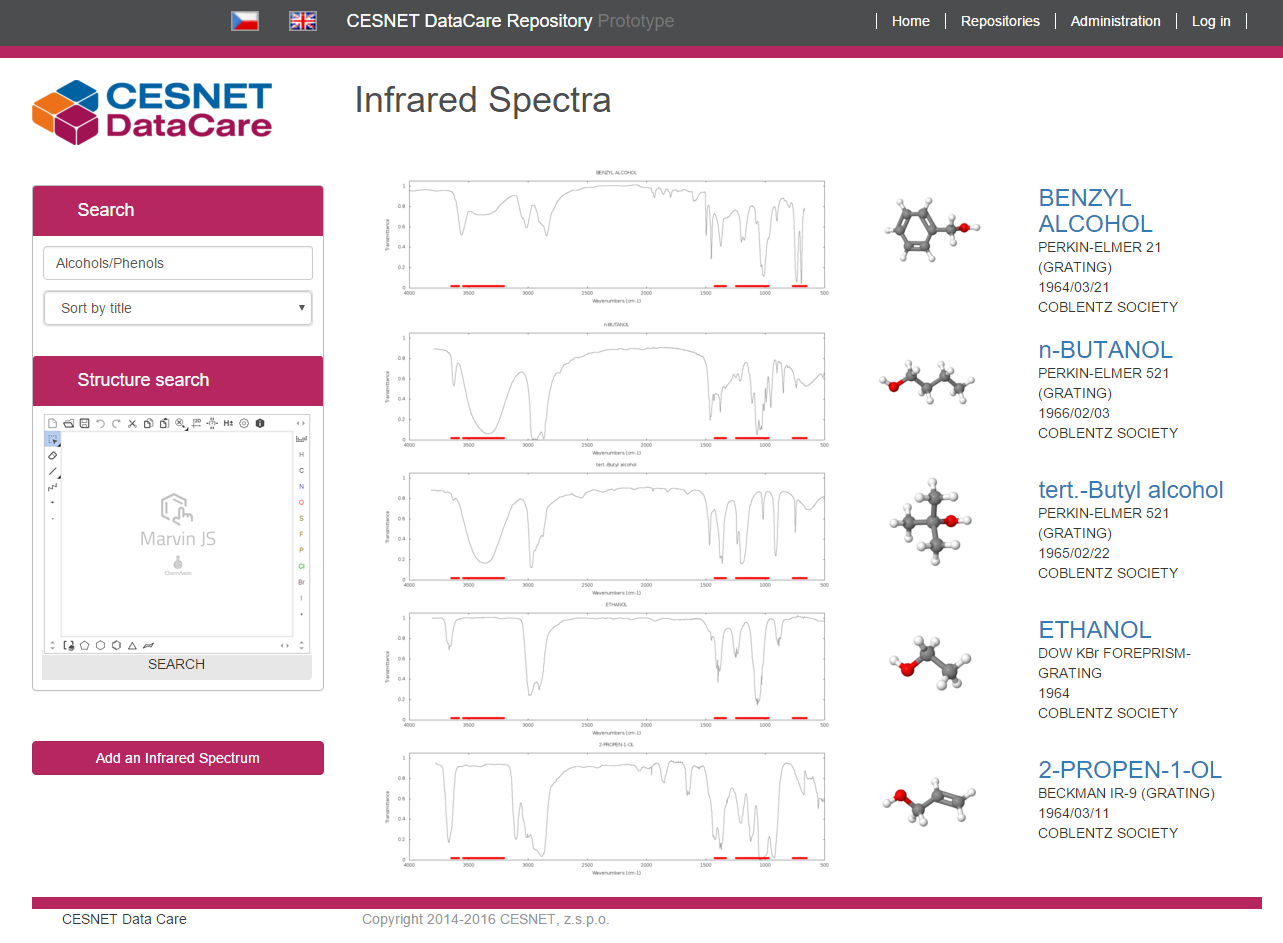
\includegraphics[width=1.0\textwidth]{grafika/list_InfraredSpectra.png}
 	\caption[Výpis dát v kolekcii InfraredSpectra]{Výpis dát v kolekcii Infrared Spectra}\label{graphics:listInfrared}
\end{figure}

\begin{figure}\centering
	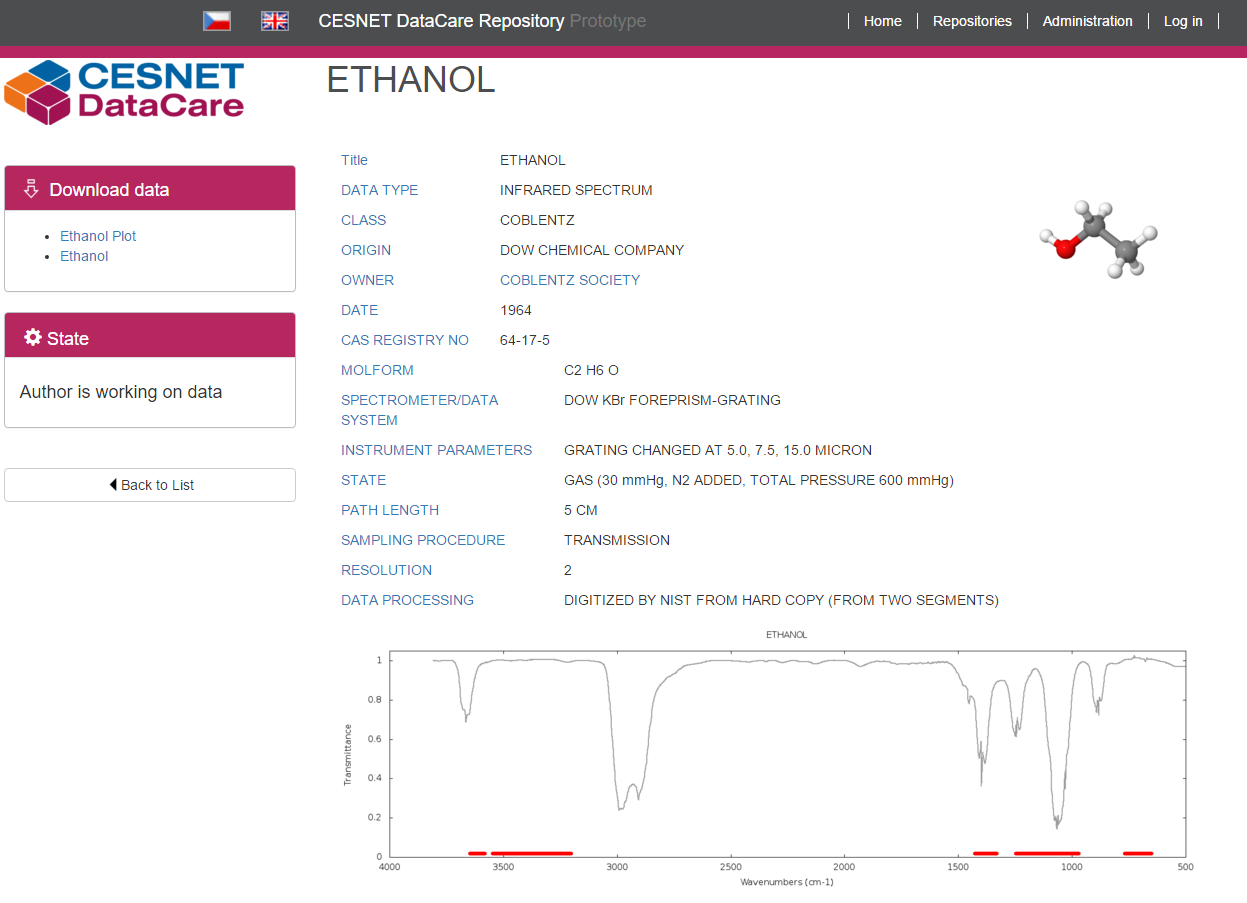
\includegraphics[width=1.0\textwidth]{grafika/detail_Ethanol.png}
 	\caption[Zobrazenie detailu konkrétnej položky (Ethanolu)]{Zobrazenie detailu konkrétnej položky (Ethanolu)}\label{graphics:Ethanol}
\end{figure}

\section{Zobrazovanie chemických dát}
Technológie, ktoré máme vybrané, Fedora a Elasticsearch, umožňujú ukladanie dát a vyhľadávanie v dátach. Fedora tiež poskytuje základné webové užívateľské rozhranie, ktoré umožňuje vytváranie nových dokumentov, zobrazenie a úpravu existujúcich. Toto webové rozhranie ale nie je užívateľsky prívetivé, taktiež je potrebné zobrazovať aj dáta v inej než textovej podobe (napríklad grafy, obrázky, štruktúru chemických látok,...), je preto potrebné vytvoriť nové webové rozhranie, ktoré umožní prácu s dokumentmi v repozitári.

Prácu s dokumentmi zjednoduší Fedoralink, ktorý tvorí medzivrstvu medzi Fedorou, Elasticsearchom a samotným webovým rozhraním napísaným v programovacom jazyku Python s využitím frameworku Django. Prácu so šablónami zase zjednodušuje fedoralink\_ui, ktorý umožňuje získavať šablóny pre jednotlivé typy dokumentov priamo z Fedora alebo z kódu aplikácie. Prečo využívam tieto technológie a ako fungujú je popísané v predchádzajúcich častiach diplomovej práce.

Pre prácu s jednotlivými dokumentmi je potrebné mať v aplikácii vytvorený model. Modely pre základné typy dokumentov sú už vytvorené vo Fedoralinku. Napríklad trieda DCObject - model pre dokumenty, ktoré obsahujú len metadáta zo schémy Dublin Core a majú priradený RDF typ DC.Object (\url{http://purl.org/dc/elements/1.1/Object}). V aplikácii fedoralink\_ui sú zase vytvorené modely potrebné pre prácu so šablónami. Napríklad trieda ResourceType, ktorá je určená pre dokumenty s RDF typom CESNET\_TYPE.ResourceType. Dokumenty s týmto RDF typom obsahujú šablóny pre zobrazenie v zozname potomkov kolekcie, zobrazenie dokumentu, editáciu dokumentu, názov a cestu k modelu v aplikácii.

Jednotlivé časti repozitára sú navrhnuté tak, aby bolo pridanie nových modelov a šablón do systému čo najjednoduchšie. Aby bolo v repozitári možné pracovať s novými typmi dokumentov (napr. s dátami z Ústavu organickej chémie VŠCHT Praha) je potrebné vytvoriť modely pre tieto dokumenty a šablóny.

\subsection{Kolekcie vo Fedore}
Dokumenty vo Fedore sú uložené buď ako kolekcie alebo binárne dáta. Dokument, ktorý je typu kolekcia môže mať pod sebou uložené ďalšie dokumenty. Vzniká teda hierarchická štruktúra, ktorá začína koreňom repozitára.

Ako prvú vec pri ukladaní nových dokumentov je potrebné vyriešiť ich hierarchické usporiadanie do rôznych kolekcií. V tejto časti diplomovej práce popisujem hierarchickú štruktúru rôznych typov dát Ústavu organickej chémie VŠCHT Praha, ktoré je potrebné ukladať, v repozitári.

\subsubsection{Inštitúcie}
Do repozitára budú môcť dáta ukladať rôzne inštitúcie. Jednotlivé dokumenty je potrebné priradiť k inštitúcii, ktorej patria. Niektoré dáta ale môžu byť zdieľané medzi viacerými inštitúciami. Preto bude vytvorená kolekcia \uv{Institutions}, v ktorej sú uložené jednotlivé inštitúcie. Ak pri jednej inštitúcii potrebujeme evidovať aj jej súčasti, tie môžu byť uložené ako potomci inštitúcie.

\subsubsection{Projekty}
Dáta, s ktorými Ústav organickej chémie VŠCHT Praha a iné inštitúcie pracujú, sú priradené k jednotlivým projektom. Na projekte môže spolupracovať niekoľko inštitúcii a vedcov. Preto je pre projekty vytvorená kolekcia \uv{Projects}, pod ňou sú uložené jednotlivé projekty.

\subsubsection{Vedci}
Vedec je osoba, ktorá sa podieľa na niektorom z projektov. Môže ale pracovať na viacerých a taktiež pracovať pre viacero inštitúcii. Preto je vytvorená samostatná kolekcia \uv{Scientists}, pod ktorou sú uložené jednotlivé osoby.

\subsubsection{Laboratórne denníky}
Laboratórne denníky Ústavu organickej chémie VŠCHT Praha, prípadne aj iných inštitúcií sú uložené pod kolekciou \uv{Laboratory journals}.

\subsubsection{Reakcie}
Reakcie, ktoré boli pozorované v rámci niektorého laboratórneho denníka sú uložené pod daným denníkom. Detaily (ako použité množstvo, koncentrácia,...) o reaktantoch a produktoch, teda chemických látkach, ktoré boli pri reakcii použité alebo pri nej vznikli, sú uložené pod touto reakciou.

\subsubsection{Chemické látky}
Samotné dáta (názov chemikálie, jej štruktúra, vlastnosti,...) o chemikáliach, ktoré môžu byť používané v rôzných reakciách, sú uložené v kolekcii \uv{Chemicals}.

\subsubsection{Analytické dáta}
NMR, IR, hmotnostné spektrá jednotlivých chemických látok a iné analytické dáta sú uložené v samostatnej kolekcii \uv{Analytical data}. Všetky zdrojové binárne dáta (výstupy zo zariadení, serializované dáta z Open Enventory,...) sú uložené v kolekcii \uv{Source data}.

Hierarchickú štruktúru kolekcií je možné vidieť na obrázku \ref{graphics:CollectionsDiagram}

\begin{figure}[h]\centering
	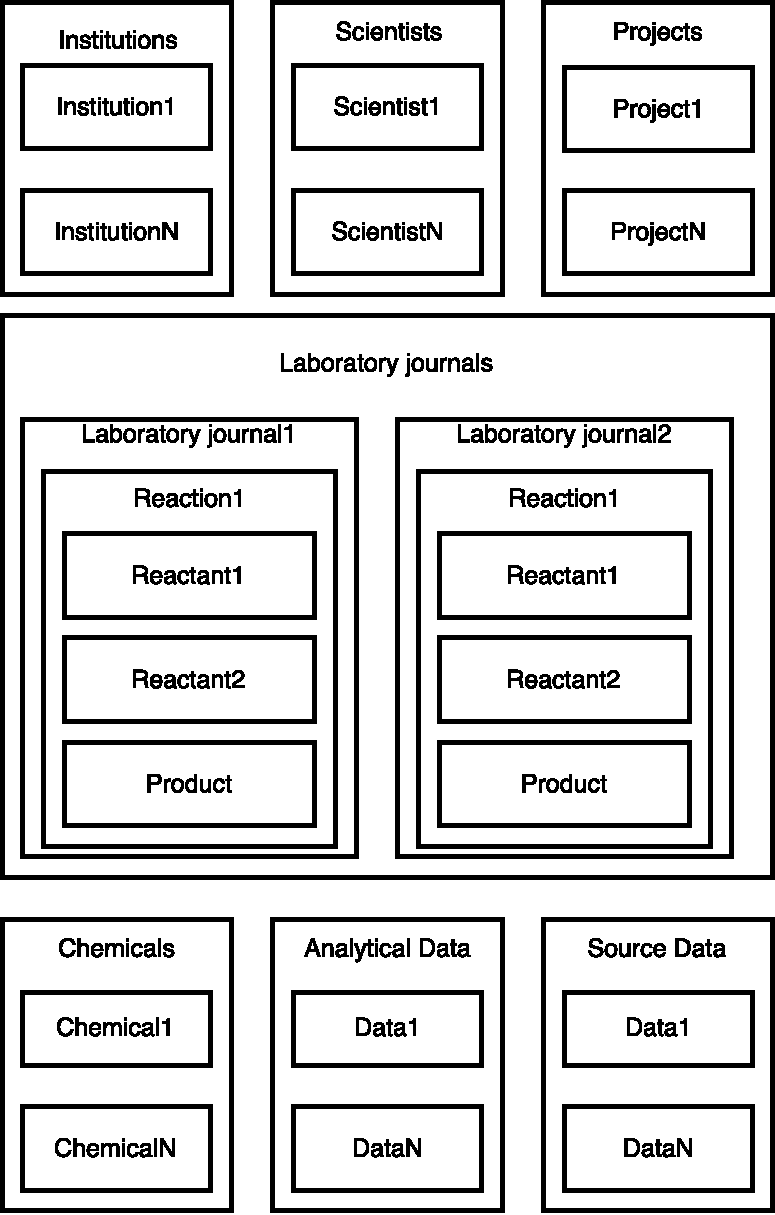
\includegraphics[width=0.8\textwidth]{diagramy/Collections_Diagram.pdf}
 	\caption[Hierarchická štruktúra kolekcií vo Fedore]{Hierarchická štruktúra kolekcií vo Fedore}\label{graphics:CollectionsDiagram}
\end{figure}

\subsection{Modely}
Modely, teda triedy pre jednotlivé dokumenty sú navrhnuté tak, aby boli čo najvšeobecnejšie, ale zároveň pokrývali všetky potrebné dáta, ktoré chcú výskumníci z Ústavu organickej chémie VŠCHT Praha v repozitári ukladať. Zároveň bolo pri ich návrhu myslené na potrebu importu dát z aplikácie Open Enventory.

V repozitári potrebujeme ukladať informácie o vedcoch, ktorí na jednotlivých projektoch pracujú. Preto bola vytvorená trieda ScientistPerson (diagram triedy je možné vidieť na obrázku \ref{graphics:ScientistPerson}).

Pre projekty je vytvorená trieda Project, ktorá okrem názvu projektu má aj odkaz na členov projektu (z modelu ScientistPerson) a tiež na inštitúcie, ktoré sa na projekte podieľajú. Trieda Institution umožňuje prácu so základnými informáciami o inštitúcii.

\begin{figure}\centering
	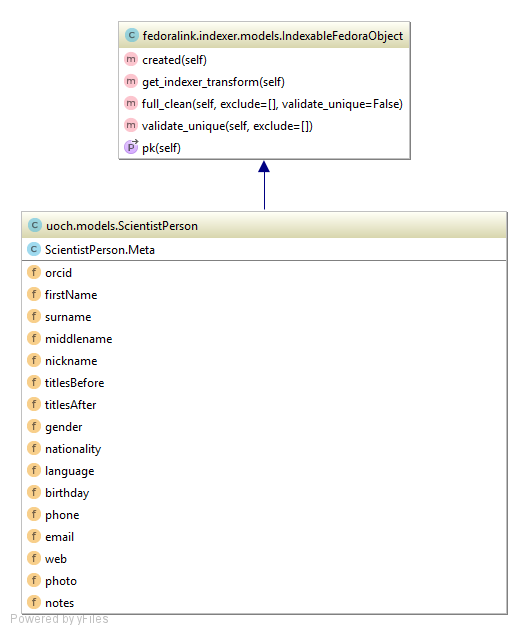
\includegraphics[width=0.9\textwidth]{diagramy/UOCH_ScientistPerson.png}
 	\caption[Model osoby - vedca]{Model osoby - vedca}\label{graphics:ScientistPerson}
\end{figure}

V laboratórnych denníkoch popisované reakcie má na starosť trieda Reaction (diagram triedy je možné nájsť na obrázku \ref{graphics:Reaction}). Medzi uložené údaje patrí popsi reakcie, pozorovanie, čas začiatku a trvanie reakcie. Reaktanty a produkty zapísané vo formáte SMILES (zjednodušený jednoriadkový zápis štruktúry). Samotné chemické látky v reakcii ale obsluhuje model ChemicalInReaction (diagram je možné vidieť na obrázku \ref{graphics:Chemical}), kde sú uvedené hodnoty ako váha, objem koncentrácia použitej látky v reakcii, či je v reakcii reaktant alebo produkt. Samotné chemické látky má na starosť trieda Chemical (\ref{graphics:Chemical})). Pri chemických látkach ukladáme hodnoty ako je štandardný názov prvku, CAS number, štruktúru chemického prvku.

\begin{figure}\centering
	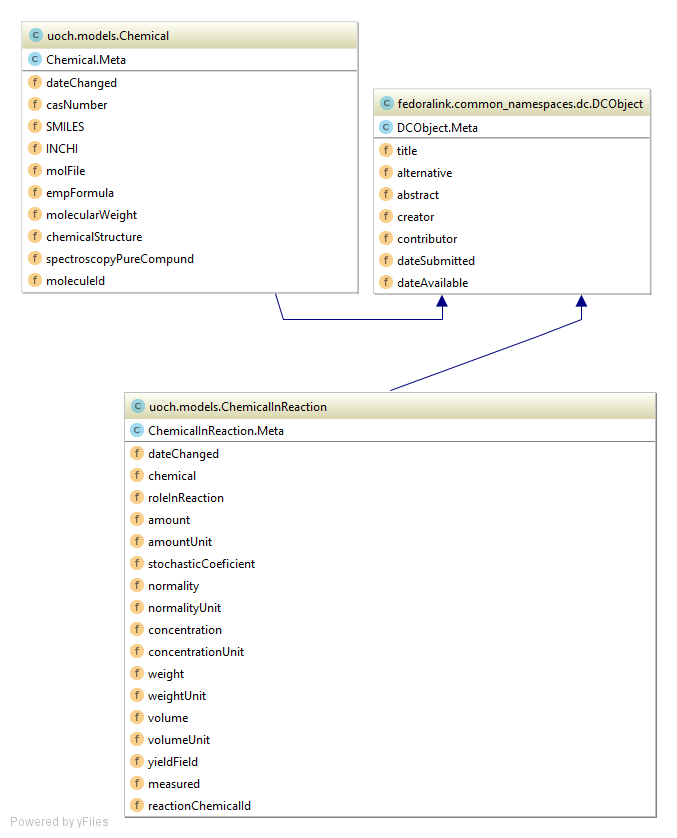
\includegraphics[width=1.0\textwidth]{diagramy/UOCH_Chemical.png}
 	\caption[Modely chemických prvkov a chemických prvkov v reakcii]{Modely chemických prvkov a chemických prvkov v reakcii}\label{graphics:Chemical}
\end{figure}

\begin{figure}\centering
	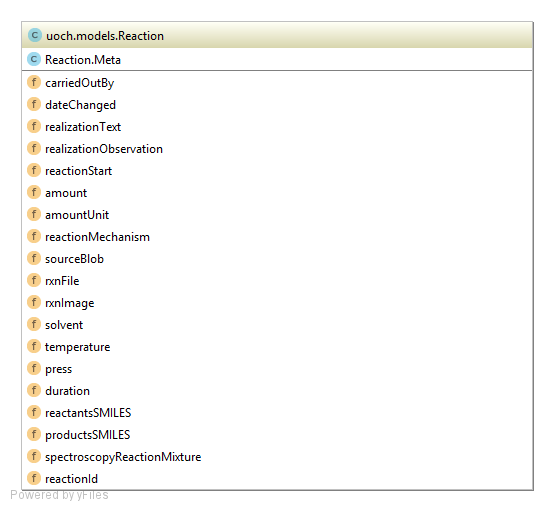
\includegraphics[width=0.9\textwidth]{diagramy/UOCH_Reaction.png}
 	\caption[Model reakcie]{Model reakcie}\label{graphics:Reaction}
\end{figure}

Analytické dáta k reakciám a chemickým látkam obsluhujú modely AnalyticalMethod, SpectroscopyMethod (napríklad NMR spektrá, IR spektrá, hmotnostné spektrá) a binárne dáta obsluhuje model SourceData a OpenEnventorySourceData (diagramy sú zobrazené na obrázku  \ref{graphics:AnalyticalMethod}). Za zdrojové dáta, ktoré ma na starosť trieda SourceData, považujeme napríklad dátové súbory s výsledkami analýz. OpenEnventorySourceData obsluhuje všetky serializované dáta k reakcii, získané importom z OpenEnventory.

\begin{figure}\centering
	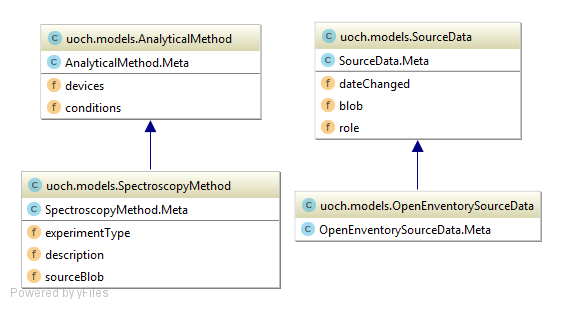
\includegraphics[width=0.9\textwidth]{diagramy/UOCH_AnalyticalMethod_and_SourceData.png}
 	\caption[Modely analytických dát a zdrojových dát]{Modely analytických dát a zdrojových dát}\label{graphics:AnalyticalMethod}
\end{figure}

\section{Automatický import dát}
Aby sme čo najviac zjednodušili vkladanie nových dát do repozitára, je potrebné upraviť niektorý z nástrojov na zber a organizáciu chemických dát, ktorý používajú výskumníci z Ústavu organickej chémie VŠCHT Praha. Pre účely diplomovej práce bol po dohode s výskumníkmi ako zdroj dát pre import vybraný nástroj Open Enventory.

Výskumníci na Ústave organickej chémie VŠCHT Praha chcú mať možnosť importovať do repozitára vybrané reakcie. K importu nemá dochádzať plne automaticky, ale až po potvrdení užívateľom. Pre tento účel je najlepšie implementovať tlačidlo umiestnené priamo vo webovej aplikácii Open Enventory. Aby bolo možné aplikáciu upraviť, je potrebné vedieť ako funguje, aké sú vzťahy medzi tabuľkami v databáze a nájsť vhodné umiestnenie pre tlačidlo.

\subsection{Schéma databázy Open Enventory}
Celá schéma databázy je na priloženom CD vo formáte UML aj SVG. V tejto časti sú popísané a okomentované databázové tabuľky, v ktorých sú uložené dáta z aplikácie Open Enventory, ktoré chceme importovať do repozitára alebo ich k tomuto importu potrebujeme.

%\begin{figure}\centering
%	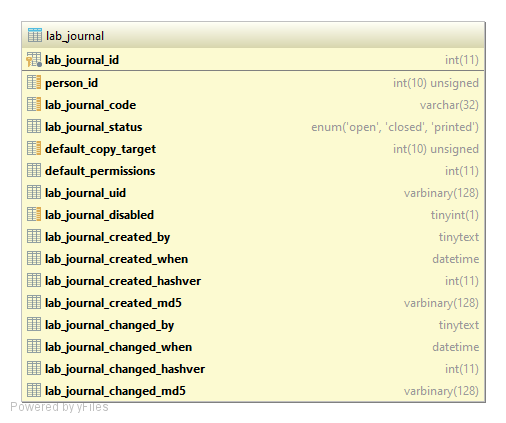
\includegraphics[width=0.8\textwidth]{Schema_DB_Open_Enventory/lab_journal.png}
% 	\caption[Štruktúra databázovej tabuľky lab\_journal]{Štruktúra databázovej tabuľky lab\_journal}\label{graphics:lab_journal}
%\end{figure}

V databázovej tabuľke lab\_journal, sú uložené základné údaje o laboratórnom denníku. Pre naše účely budú ďalej dôležité stĺpce person\_id a primárny kľúč lab\_journal\_id.

%\begin{figure}\centering
%	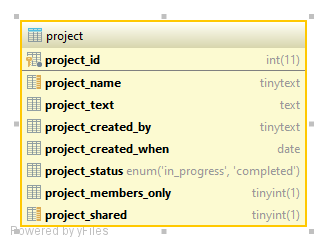
\includegraphics[width=0.6\textwidth]{Schema_DB_Open_Enventory/project.png}
% 	\caption[Štruktúra databázovej tabuľky project]{Štruktúra databázovej tabuľky project}\label{graphics:project}
%\end{figure}

V rámci laboratórnych denníkov sú vytvorené jednotlivé projekty užívateľov.

\begin{figure}\centering
	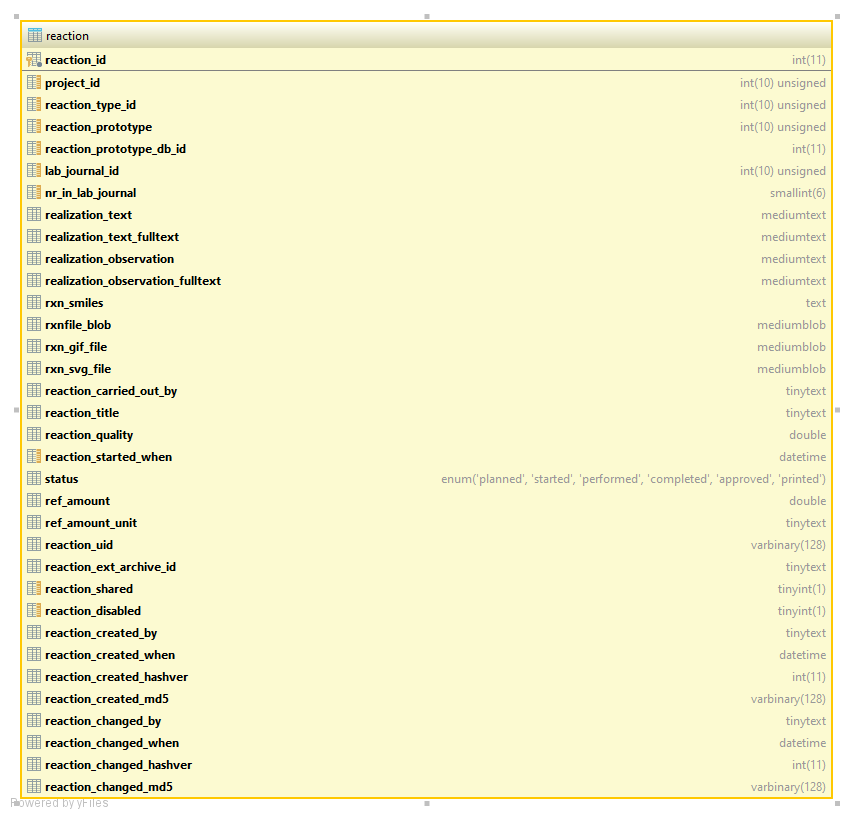
\includegraphics[width=1.0\textwidth]{Schema_DB_Open_Enventory/reaction.png}
 	\caption[Štruktúra databázovej tabuľky reaction]{Štruktúra databázovej tabuľky reaction}\label{graphics:reaction}
\end{figure}

Samotné dáta meraní, popis a priebeh reakcií sú uložené v databázovej tabuľke reaction, jej schému si je možné pozrieť na obrázku \ref{graphics:reaction}. Tá je cez stĺpec project\_id prepojená s tabuľkou project a cez stĺpec lab\_journal\_id s tabuľkou lab\_journal. Zároveň má každá reakcia jedinečné poradové číslo v denníku uložené v stĺpci nr\_in\_lab\_journal.

Popis reakcie je uložený v stĺpci realization\_text\_fulltext, pozorovanie v sĺpci realization\_observation\_fulltext, množstvo výslednej látky v stĺpci ref\_amount a jednotka, v akej je toto množstvo uvedené, v stĺpci ref\_amount\_unit. Ďalšie namerané hodnoty sú ako binárné hodnoty uložené v stĺpcoch rxnfile\_blob, rxn\_gif\_file - chemická rovnica reakcie vo formáte GIF, rxn\_svg\_file - obrázok vo formáte SVG. RXN je formát pre popis reakcie, ktorý pozostáva z bloku reaktantov, produktov a prípadne (nie veľmi zvyčajne) aj bloku agentov.

Ďalšie dáta ako doba trvania reakcie, použité rozpúšťadlo a jeho koncentrácia alebo teplota, pri ktorej reakcia prebiehala, sú uložené v tabuľke reaction\_property. V stĺpci reaction\_property\_name je uložený názov vlastnosti (napríklad \uv{solvent} teda rozpúšťadlo, \uv{temperature} teda teplota, ...) a v stĺpci reaction\_property\_value je uložená samotná hodnota.

V tabuľke analytical\_data (schéma je na obrázkoch \ref{graphics:analyticalData1} a \ref{graphics:analyticalData2}) sú uložené rôzne analýzy reakcie a chemických prvkov. Analytické dáta môžu byť H NMR spektrá, C NMR spektrá, teda spektroskopia nukleárnej magnetickej rezonancie s využitím vodíka alebo uhlíka; infračervené spektrá, hmotnostné spektrá. Do Open Enventory mohli byť tieto analýzy uložené v binárnom formáte (väčšinou ako dokument vo formáte PDF alebo obrázok vo formáte TIF, RAW), v databázovej tabuľke sa okrem binárnych hodnôt nachádzajú grafy (obrázky) k jednotlivým analytickým dátam. Tieto grafy/obrázky sú uložené v stĺpci  analytical\_data\_graphics\_blob, textová interpretácia dát (ak je možná) v stĺpci analytical\_data\_interpretation, komentár k dátam v stĺpci analytical\_data\_comment. Pôvodné dáta su uložené v stĺpci analytical\_data\_raw\_blob, kde sú súbory uložené do archívu TAR a komprimované metódou gzip. Prepojenie na tabuľku reaction\_chemical je cez stĺpec reaction\_chemical\_id.

\begin{figure}\centering
	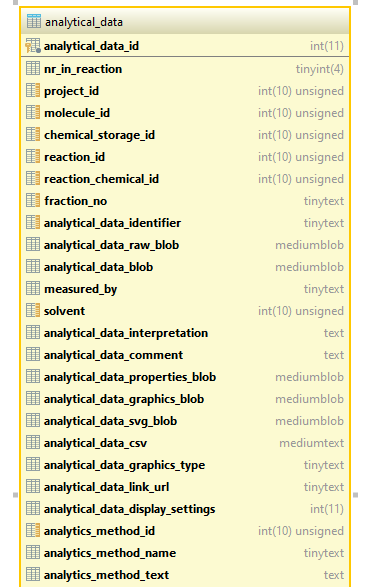
\includegraphics[width=0.7\textwidth]{Schema_DB_Open_Enventory/analytical_data1.png}
 	\caption[Štruktúra databázovej tabuľky analytical\_data, 1. časť]{Štruktúra databázovej tabuľky analytical\_data, 1. časť}\label{graphics:analyticalData1}
\end{figure}

\begin{figure}\centering
	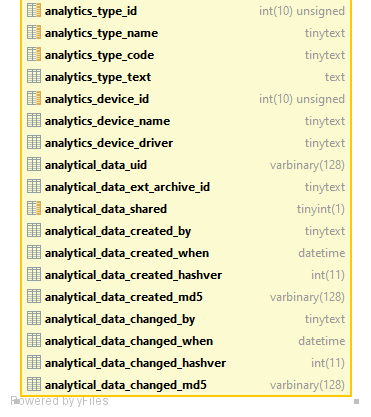
\includegraphics[width=0.7\textwidth]{Schema_DB_Open_Enventory/analytical_data2.png}
 	\caption[Štruktúra databázovej tabuľky analytical\_data, 2. časť]{Štruktúra databázovej tabuľky analytical\_data, 2. časť}\label{graphics:analyticalData2}
\end{figure}

\begin{figure}\centering
	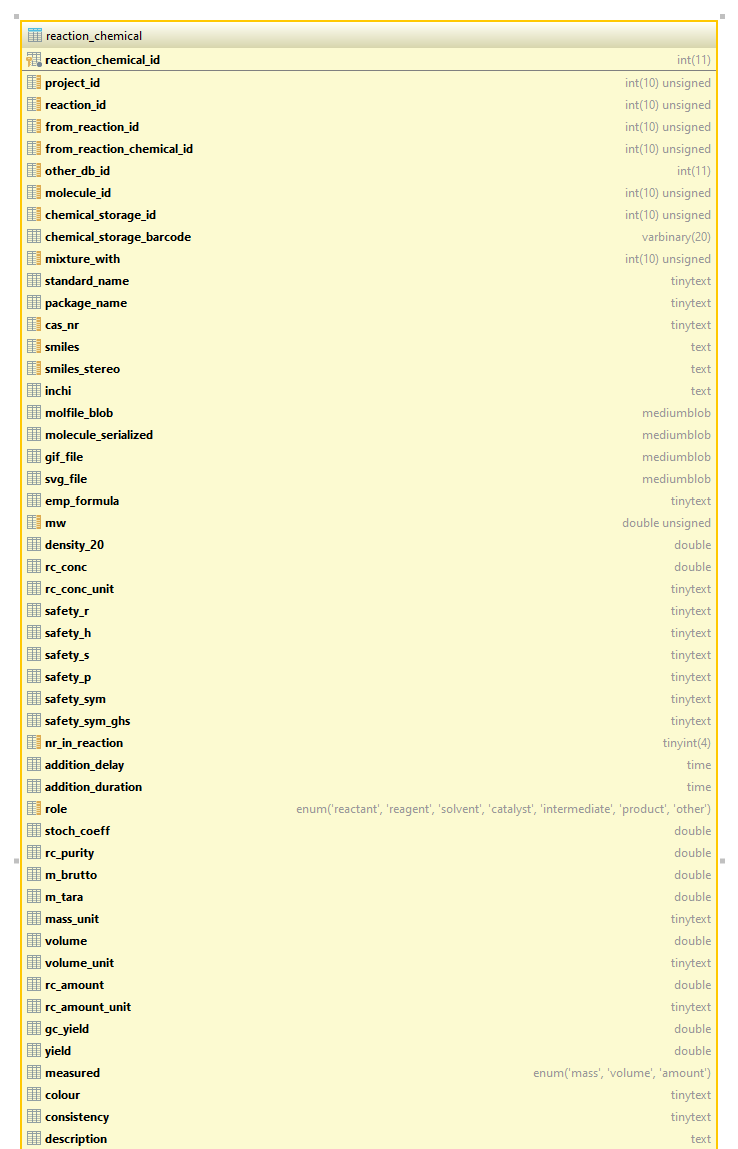
\includegraphics[width=1.0\textwidth]{Schema_DB_Open_Enventory/reaction_chemical_1.png}
 	\caption[Štruktúra databázovej tabuľky reaction\_chemical, 1. časť]{Štruktúra databázovej tabuľky reaction\_chemical, 1. časť}\label{graphics:reactionChemical1}
\end{figure}

\begin{figure}\centering
	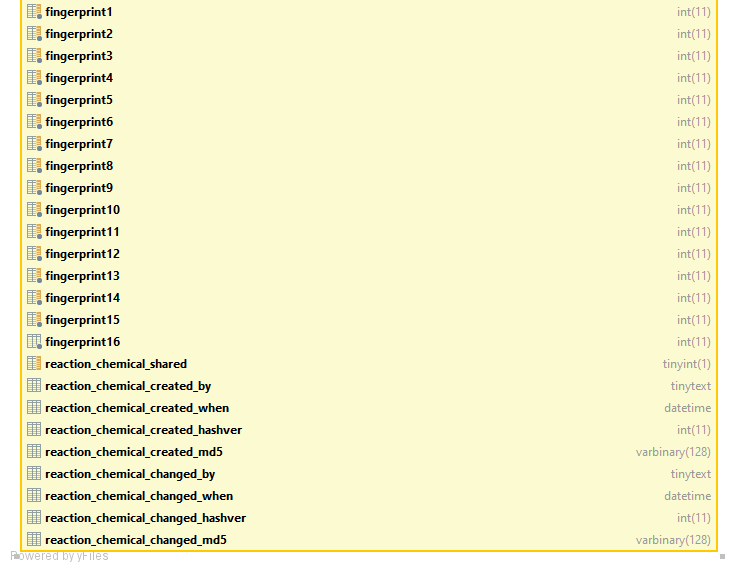
\includegraphics[width=1.0\textwidth]{Schema_DB_Open_Enventory/reaction_chemical_2.png}
 	\caption[Štruktúra databázovej tabuľky reaction\_chemical, 2. časť]{Štruktúra databázovej tabuľky reaction\_chemical, 2. časť}\label{graphics:reactionChemical2}
\end{figure}

V tabuľke reaction\_chemical (schéma je na obrázkoch \ref{graphics:reactionChemical1} a \ref{graphics:reactionChemical2}) sú uložené informácie o reaktantoch a produktoch. Môže tu byť uvedený štandardný názov prvku v stĺpci standard\_name, tzv. SMILES teda zjednodušený jednoriadkový zápis štruktúry (uložené v sĺpci smiles). Binárne hodnoty popisujúce prvok v stĺpcoch molfile\_blob (MDL Molfile je súborový formát, ktorý umožňuje ukladať informácie o atómoch, spojeniach, prepojeniach a polohe molekúl), molecule\_serialized, gif\_file - obsahuje obrázok štruktúry prvku vo formáte GIF, svg\_file - štruktúra prvku na obrázku vo formáte SVG.

Chemický vzorec prvku je uložený v stĺpci emp\_formula, molekulárna hmotnosť v stĺpci mw, poradie reaktantov a produktov je v stĺpci nr\_in\_reaction. Či ide o reaktant alebo produkt, sa dozvieme zo stĺpca role. Stochastický koeficient v stĺpci stoch\_coeff, hmotnosť v stĺpci m\_brutto, jednotka, v akej je hmotnosť uvedená, je v stĺpci mass\_unit, objem v stĺpci volume a jednotka objemu v stĺpci volume\_unit. Koncentrácia v stĺpci rc\_amount a jednotka, v akej je koncentrácia uvedená, je v stĺpci rc\_amount\_unit.
V prípade produktov je v stĺpci yield uložené reálne získané množstvo v \% a z rc\_amount sa dá zistiť teoreticky získateľná koncentrácia.

\subsection{Implementácia automatického importu}
Štruktúru databázových tabuliek a prepojenia medzi nimi už poznáme, ďalej sa bolo potrebné rozhodnúť na spôsobe implementácie automatického importu dát z Open Enventory do repozitára.

Do úvahy prichádzajú dve možnosti:
\begin{enumerate}
	\item Implementácia v programovacom jazyku PHP, ktorá by bola priamo súčasťou Open Enventory. Autor Open Enventory ale na získavanie dát využíva volania z javascriptu, kde jednotlivé hodnoty získava postupne. Nemá tu teda v PHP pripravené objekty ani funkcie, ktoré by získanie laboratórnych denníkov uľahčili. Kód aplikácie je naviac neprehľadný s komentármi a aj časťou kódu v nemeckom jazyku.
	\item Implementácia samostatného skriptu s napojením priamo na databázu, ktorý by sa staral o automatický import dát do repozitára. V samotnom Open Enventory je v tomto prípade potrebné umiestniť tlačidlo, ktoré spustí tento skript a predá mu parametre potrebné pre import (teda id reakcie alebo laboratórneho denníka, ktorý chce užívateľ importovať do repozitára).
\end{enumerate}

Rozhodol som sa pre druhú možnosť, pričom využívam programovací jazyk Python a framework Django. Django, po nastavení pripojenia k databáze, umožňuje automatické vytvorenie modelov pre tabuľky v databáze. Vzhľadom na nezadefinované cudzie kľúče a ďalšie zistené chyby, bolo pre ľahšiu prácu s modelmi potrebné vygenerované triedy upraviť.

\section{Kontrola stavov a prístupové práva} \label{stavy}
Fedora umožňuje nastaviť práva pre jednotlivé dokumenty pomocou ACL. Takýmto spôsobom vieme nastaviť, kto môže daný dokument zobraziť, kto ho môže upraviť... Keďže má byť repozitár pre užívateľov čo najjednoduchší, nie je takéto nastavovanie prístupových práv ideálne. Tieto práva by bolo potrebné nastavovať a hlavne meniť pre každý dokument individuálne. Tak by mohlo dochádzať k častým chybám s nesprávne nastavenými oprávneniami. Preto bol navrhnutý spôsob kontroli prístupových práv cez stavy. Tieto určujú v akom stave alebo stavoch sa konkrétny dokument nachádza.

Napríklad môže ísť o schvaľovací proces. Vložené dáta nesmú byť zverejnené hneď. Je potrebné, aby prešli procesom schvalovania cez viacero ľudí. Prístup k tomuto dokumentu má na začiatku osoba, ktorá dokument vytvorila, tá môže požiadať o jeho zverejnenie. Zmení sa stav a nové nastavenie prístupových práv umožní, aby dáta videli aj osoby, ktoré majú právo schváliť zverejnenie. Po schválení všetkými potrebnými osobami dôjde opäť ku zmene stavu a prístupu k týmto dátam. Keď sa dokument nachádza v stave \uv{zverejnený}, prezerať si ho môžu všetci. Právo na editáciu ale ostane len pôvodnému autorovi prípadne editorovi. Po úprave bude ale opäť potrebné požiadať o schválenie.

Možnosti Fedory, nutné úpravy a detailnejšie informácie o stavoch sú popísané nižšie.

\subsection{Prístupové práva vo Fedore}
Fedora 4 obsahuje modul WebAC Authorization Delegate, ktorý je implementáciou W3C návrhu decentralizovaného autorizačného mechanizmu na základe RDF. Tento mechanizmus sa nazýva WebAccessControl \url{https://www.w3.org/wiki/WebAccessControl}.

\subsubsection{WebAccessControl}
Je decentralizovaný systém umožňujúci rôznym užívateľom a skupinám rozdielne prístupy k dokumentom na základe identifikácie užívateľov a skupín cez HTTP URI. 

Takýmto spôsobom je možné nastaviť prístup k dokumentu uloženom na jednom mieste užívateľom a skupinám hostovaným na inom mieste. Užívateľ tak nemusí mať vytvorený profil na mieste, kde je dokument uložený.

Každý dopyt na webový zdroj vráti HTTP dokument obsahujúci hlavičku s odkazom na ACL dokument, ktorý popisuje prístupové práva pre daný dokument (prípadne pre iné dokumenty).
\cite{WebAccessControl}

Nastavenie prístupových práv, prepojenie dokumentov a ACL dokumentov je možné vidieť na diagrame znázornenom na obrázku \ref{graphics:WebACL}. Podľa diagramu je umožnený prístup na čítanie všetkým, kto pristupujú k dokumentu /2013/card, ale k dokumentu /2013/protected majú prístup len užívatelia, ktorý patria do skupiny conf.example (teda účastníci konferencie).

\begin{figure}\centering
	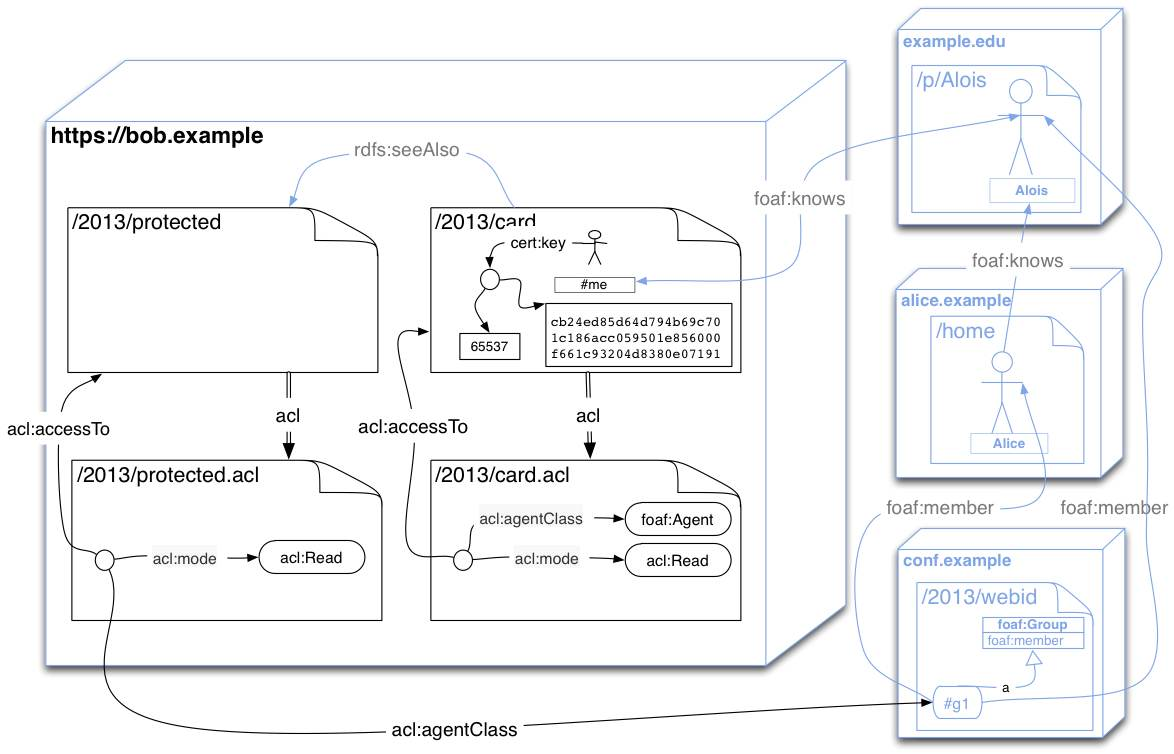
\includegraphics[width=1.0\textwidth]{stavy/WebACL.jpg}
 	\caption[Diagram WebACL]{Diagram prístupových práv, prepojenia dokumentov a ACL dokumentov, zdroj: \cite{WebAccessControl}}\label{graphics:WebACL}
\end{figure}

ACL je zoznam oprávnení priradených k nejakému dokumentu. Pomocou ACL môžeme určiť, ktoré osoby (parameter {\em agent}) alebo skupiny (parameter {\em agentClass}) majú mať prístup k danému dokumentu. Tento dokument, prípadne dokumenty sú určené parametrom {\em accessTo} alebo {\em accessToClass}. Ako trieda pre všetkých užívateľov sa štandardne používa foaf:Agent a znamená, že dokument je verejne dostupný.
Typ prístupu je určený parametrom {\em mode}. Typy prístupu sú popísané v tabuľke \ref{tab:modeACL}.

\begin{table}[!htbp]\centering
 	\caption[Typy prístupu v ACL]{Typy prístupu v ACL}\label{tab:modeACL}
\begin{tabularx}{\textwidth}{|l|X|} \hline
Read	        & Oprávnenie na čítanie obsahu \\ \hline
Write 	& Oprávnenie na prepísanie obsahu \\ \hline
Append	& Oprávnenie na pridanie informácie (na koniec už existujúcej, nedáva právo na zmazanie)  \\ \hline
Control	& Oprávnenie na nastavenie prístupu na seba (prístup k danému ACL) \\ \hline
\end{tabularx}
\end{table} 

Príklad nastavenia prístupu (vo formáte turtle\footnote{Turtle je definicia textovej syntaxe, ktorá umožňuje zápis celého RDF grafu v textovej podobe. \cite{RDF}\nopagebreak}):
\begin{lstlisting}[frame=single] 
@prefix acl: <http://www.w3.org/ns/auth/acl#> .

<> a acl:Authorization;
    acl:accessTo <$FCREPOREL/administration/states>;
    acl:agentClass <$FCREPOREL/groups/groupAll>;
    acl:mode acl:Read.
\end{lstlisting}
Toto ACL umožní prístup na čítanie k dokumentu s URI /administration/states v repozitári pre všetkých členov skupiny groupAll (zoznam členov tejto skupiny máme uložený na adrese /groups/groupAll). \$FCREPOREL je relatívna cesta ku koreňu repozitára.

\subsubsection{Proces získania oprávnení pre dokument vo Fedore}
Proces získania oprávnení je znázornený na diagrame \ref{graphics:ACLFedoraFlow}. Užívateľ, ktorý môže patriť do nejakej skupiny, požiada o prístup k dokumentu uloženému vo Fedore. Dokument môže mať priradený typ. Fedora zistí, či k danému dokumentu existuje ACL (dokument má nastavený parameter acl:AccessControl). Ak nie, prejde všetkých rodičov až po koreň. Pokiaľ ACL nenájde, prístup k danému dokumentu zakáže.
V opačnom prípade zistí, či má užívateľ prístup na daný dokument, na daný typ dokumentov alebo či má oprávnenie užívateľova skupina. Ak nenájde žiadne oprávnenie, prístup zakáže, inak vráti dopytovaný dokument.

\begin{figure}\centering
	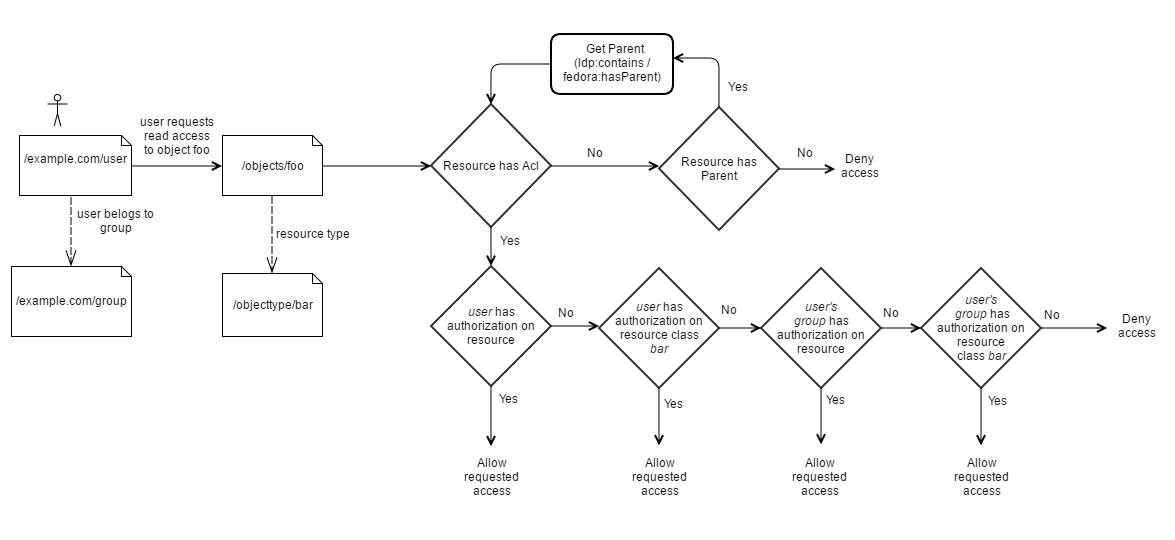
\includegraphics[width=1.0\textwidth]{stavy/ACLFedoraFlow.png}
 	\caption[Proces získania oprávnení vo Fedore]{Proces získania oprávnení vo Fedore, zdroj: \cite{FedoraACL}}\label{graphics:ACLFedoraFlow}
\end{figure}

\subsection{Stavy}
Aby bola práca užívateľov s repozitárom čo najviac zjednodušená, každý dokument v repozitári môže mať definovaný stav. Ten následne určuje oprávnenia pre prístup k danému dokumentu.

\subsubsection{Stav uloženého dokumentu v repozitári}
Stav je k dokumentu priradený pomocou parametru state:State. V jednom okamžiku môže mať dokument priradených aj viacero stavov (parameter state:State je v takom prípade použitý viackrát).

Takýto stav môže napríklad vyjadrovať stav schvaľovania publikovania dát. Nový dokument, ktorý chce autor zverejniť, je potrebné schváliť vedúcim pracovníkom. Dokument sa nachádza v stave, kedy čaká na zverejnenie. Prístup k nemu v danej chvíli má jeho autor a osoba, ktorá má zverejnenie potvrdiť.

Stavy, v ktorých sa môže nejaký dokument nachádzať, sú uložené v kolekcii stavov. Tá je k danému dokumentu priradená parametrom state:stateControl.

Príklad dokumentu s priradenými stavmi:
\begin{lstlisting}[frame=single] 
@prefix acl: <http://www.w3.org/ns/auth/acl#>.
@prefix state: <http://cesnet.cz/ns/repository/state#>.
@prefix dc: <http://purl.org/dc/elements/1.1/>.

<> acl:accessControl </fcrepo/rest/acl>;
   state:stateControl </fcrepo/rest/states>;
   state:State </fcrepo/rest/states/wg1_approving>,
               </fcrepo/rest/states/wg2_approving>;
   dc:title "Hello, World!".
\end{lstlisting}

\subsubsection{Stav}
Stav je dokument typu state:State, ktorý je uložený v kolekcii stavov v repozitári. Pre stav sú definované prístupové práva (ACL). Aby bolo možné zmeniť stav, v akom sa nejaký dokument nachádza, je potrebné taktiež definovať povolené zmeny stavov.

\begin{itemize}
	\item state:defaultAccessControl definuje ACL pre dokumenty s týmto stavom.
	\item state:allowedStateTransitions definuje povolené zmeny stavov. Ako hodnota tohto parametra je dokument typu state:Transition.
\end{itemize}

\subsubsection{Prechod medzi stavmi}
Dokument typu state:Transition definuje prechod medzi dvoma stavmi a práva, kto môže danú zmenu realizovať.

State:targetState určuje cieľový stav prechodu.
ACL priradené na dokument typu state:Transition určuje, kto môže zmenu realizovať.

\subsection{Stavy vo Fedore}
Vo Fedore žiadne stavy ani nástroje na kontrolu stavov a prechodov medzi nimi neexistujú. Aplikáciu je teda potrebné upraviť tak, aby takúto kontrolu umožňovala.

Pri každom dopyte do Fedory potrebujeme skontrolovať, či dochádza k zmene stavu dokumentu. V prípade, ak áno, je potrebné skontrolovať oprávnenia a zmenu povoliť alebo zamietnuť. K ukladaniu upravených dokumentov dochádza vo funkcii patchResourcewithSparql v triede ContentExposingResource.
K volaniu tejto funkcie ale dochádza z objektu, ktorý je typu FedoraLdp. Trieda FedoraLdp dedí z triedy ContentExposingResource. Obe sa nachádzajú v module fcrepo-http-api.

Fedora sa stále rýchlo vyvíja. Aktuálne vývojári pracujú aj na API-X, ktoré umožní rozširovanie kódu Fedory. Momentálny stav vývoja API-X však neumožňuje jeho využitie pre úpravu potrebného kódu. Upravovať priamo kód modulu fcrepo-http-api by spôsobilo komplikácie pri aktualizácii Fedory, ale taktiež pri šírení takto upravenej verzie. Vytvoril by som v podstate novú vetvu vývoja Fedory, pričom by bolo pri vydaní novej verzie Fedory robiť zlúčenie medzi vetvami. Čo by mohlo byť vzhľadom na možné zmeny kódu aj v časti, ktorú potrebujem upraviť, komplikované.

Menej často sa menia rozhrania metód a ich parametre, to je možné využiť, ak existuje nástroj, ktorý umožňí rozšírenie existujúceho kódu mimo kódu Fedory. Riešením je vytvorenie Java aplikácie využívajúcej rozšírenie AspectJ. Pri správnom nastavení Mavenu vytvorí nový modul fcrepo-http-api obsahujúci upravený kód. V skompilovanej Fedore následne stačí vymeniť súbor fcrepo-http-api.jar za novovytvorený fcrepo-http-api-with-states.jar.

\subsubsection{AspectJ}
V programovaní sa často využíva proces oddelenia zodpovedností (v angličtine Separation of concerns - SoC), ide o snahu rozdeliť program do samostatných častí, z ktorých každá má inú funkciu. Funkcie a kódy jednotlivých častí by sa mali čo najmenej prekrývať. O takéto oddelenie zodpovedností sa snaží aj aspektovo orientované programovanie (AOP).

Vysvetlenie používaných termínov:
\begin{itemize}
	\item Extension methods - umožňujú pridať metódy, premenné a rozhrania do existujúcej triedy v rámci aspektu.
	\item Pointcut - umožňuje definovať tzv. join points, teda presne definované miesta v bežiacom programe (ako sú volania metód, inicializácia objektov alebo prístup k premenným).
	\item Advices - kód, ktorý sa spustí po splnení podmienky špecifikovanej v pointcute. Tento kód môže byť spustený pred, po alebo okolo definovaného miesta v bežiacom programe.
	\item Weaving - proces vkladania aspektov do aplikácie.
	\item Aspekt - je kombináciou advice a pointcutu, umožňuje teda spustiť kód na presnom mieste v bežiacej aplikácii.
\end{itemize}
Vďaka aspektom môžeme upraviť chovanie programu na presne definovanom mieste. Takéto aspekty sa často využívajú k logovaniu, umožňujú spúšťať jeden kód na viacerých miestach programu, pričom nie je potrebné meniť samotný kód programu. V prípade potrebných zmien stačí kód pre logovanie upraviť na jednom mieste. \cite{aspect} V mojom prípade bude vďaka aspektom možné upraviť kód pre ukladanie upravených objektov do Fedory tak, aby kontroloval zmenu stavov a oprávnenia pre ich zmenu.

AspectJ \url{http://www.eclipse.org/aspectj/} je rozšírenie využívajúce aspektovo orientované programovanie pre jazyk Java. Toto rozšírenie umožňuje využívať aspekty.

Konfigurácia AspectJ je uložená v súbore aop.xml
\lstset{language=XML}
\begin{lstlisting}[frame=single] 
<!DOCTYPE aspectj PUBLIC "-//AspectJ//DTD//EN" "http://www.eclipse.org/aspectj/dtd/aspectj.dtd">

<aspectj>

    <weaver options="-verbose -showWeaveInfo">
        <include within="org.fcrepo.http.api.FedoraLdp"/>
        <include within="org.fcrepo.http.api.ContentExposingResource"/>
        <include within="org.fcrepo.http.api.FedoraBaseResource"/>
    </weaver>

    <aspects>
        <aspect name="cz.cesnet.fcrepo.interceptor.PatchWrapAspect"/>
    </aspects>

</aspectj>
\end{lstlisting}
V časti weaver je nastavený spôsob weavingu. Potrebujeme mať prístup k triedam FedoraLdp, ContentExposingResource a FedoraBaseResource, ktoré od seba dedia.

Kód aspektu, ktorý sa spustí pri každom volaní metódy patchResourcewithSparql:
\lstset{language=Java}
\begin{lstlisting}[frame=single] 
@SuppressWarnings("PackageAccessibility")
public privileged aspect PatchWrapAspect {
    @Inject
    protected Session session;

    public pointcut wrapPatch(FedoraResource resource, String requestBody, RdfStream resourceTriples) :
    execution(* patchResourcewithSparql(FedoraResource, java.lang.String, RdfStream)) && this(org.fcrepo.http.api.FedoraLdp) && args(resource, requestBody, resourceTriples);

    Object around(FedoraResource resource, String requestBody, RdfStream resourceTriples) : wrapPatch(resource, requestBody, resourceTriples) {
        try {
            ContentExposingResource currentResource = (ContentExposingResource) thisJoinPoint.getThis();
            HttpSession session = currentResource.session;
            ContainerRequestContext request = (ContainerRequestContext) currentResource.request;
            IdentifierConverter<Resource, FedoraResource> translator = currentResource.translator();

            final UpdateRequest update_request = UpdateFactory.create(requestBody,
                    translator.reverse().convert(resource).toString());

            StateAuthorizationDelegate sad = new StateAuthorizationDelegate(this.session, translator,
                    session.getFedoraSession().getUserId());

            requestBody+= sad.checkState(resource, update_request);

            return proceed(resource, requestBody, resourceTriples);
        }
        catch (RuntimeException e){
            e.printStackTrace();
            System.out.println(e.getMessage());
            throw e;
        }
    }
}
\end{lstlisting}

\subsection{Kontrola stavov}
S využitím aspektu po nahradení pôvodného kódu potrebujeme zistiť, či sa niekto pokúša zmeniť StateControl upravovaného dokumentu. V prípade ak to robí užívateľ, ktorý nemá oprávnenie na zmenu, aplikácia vráti chybový HTTP kód.
Ak StateControl nie je k dokumentu priradený, ale užívateľ sa pokúša priradiť k dokumentu stavy, aplikácia taktiež vráti chybový HTTP kód.

Ak je StateControl upraveného dokumentu a pôvodného rovnaký, porovnáme stavy. Ak došlo k zmene v stavoch, je potrebné získať všetky povolené prechody z pôvodných stavov. Keďže operáciu, pri ktorej získavame dokumenty typu StateTransition, robí aplikácia pod užívateľom, ktorý poslal dopyt, získa len prechody, ktoré má daný užívateľ povolené.
Po získaní možných cieľových stavov z týchto prechodov, aplikácia zistí, či sa medzi nimi nachádza každý nový cieľový stav. Ak niektorý z nových stavov nie je medzi povolenými cieľovými stavmi pre daného užívateľa, aplikácia vráti chybový kód.

Ak sú povolené všetky nové stavy, aplikácia upraví pôvodný dopyt tak, aby sa všetky pôvodné stavy zmazali.

\begin{conclusion}
	%sem napíšte záver Vašej práce
\end{conclusion}

\bibliographystyle{csn690}
\bibliography{mybibliographyfile}

\appendix

\chapter{Zoznam použitých skratiek}
% \printglossaries
\begin{description}
	\item[VŠCHT] Vysoká škola chemicko-technologická
	\item[CIS] Centrum informačných služieb
	\item[ELN] Electronic lab notebook
	\item[GUI] Graphical user interface
	\item[XML] Extensible markup language
	\item[RDF] Resource Description Framework
	\item[ACL] Access control list
	\item[UML] Unified Modeling Language
	\item[SVG] Scalable Vector Graphics
	\item[GIF] Graphics Interchange Format
	\item[SMILES] simplified molecular-input line-entry system
	\item[HTTP] Hypertext Transfer Protocol
	\item[URI] Uniform Resource Identifier
	\item[URL] Uniform Resource Location
	\item[AOP] Aspect-oriented programming
	\item[TAR] Tape archiver
	\item[GZIP] GNU zip
\end{description}


% % % % % % % % % % % % % % % % % % % % % % % % % % % % 
% % Tuto kapitolu z výsledné práce ODSTRAŇTE.
% % % % % % % % % % % % % % % % % % % % % % % % % % % % 
% 
% \chapter{Návod k~použití této šablony}
% 
% Tento dokument slouží jako základ pro napsání závěrečné práce na Fakultě informačních technologií ČVUT v~Praze.
% 
% \section{Výběr základu}
% 
% Vyberte si šablonu podle druhu práce (bakalářská, diplomová), jazyka (čeština, angličtina) a kódování (ASCII, \mbox{UTF-8}, \mbox{ISO-8859-2} neboli latin2 a nebo \mbox{Windows-1250}). 
% 
% V~české variantě naleznete šablony v~souborech pojmenovaných ve formátu práce\_kódování.tex. Typ může být:
% \begin{description}
% 	\item[BP] bakalářská práce,
% 	\item[DP] diplomová (magisterská) práce.
% \end{description}
% Kódování, ve kterém chcete psát, může být:
% \begin{description}
% 	\item[UTF-8] kódování Unicode,
% 	\item[ISO-8859-2] latin2,
% 	\item[Windows-1250] znaková sada 1250 Windows.
% \end{description}
% V~případě nejistoty ohledně kódování doporučujeme následující postup:
% \begin{enumerate}
% 	\item Otevřete šablony pro kódování UTF-8 v~editoru prostého textu, který chcete pro psaní práce použít -- pokud můžete texty s~diakritikou normálně přečíst, použijte tuto šablonu.
% 	\item V~opačném případě postupujte dále podle toho, jaký operační systém používáte:
% 	\begin{itemize}
% 		\item v~případě Windows použijte šablonu pro kódování \mbox{Windows-1250},
% 		\item jinak zkuste použít šablonu pro kódování \mbox{ISO-8859-2}.
% 	\end{itemize}
% \end{enumerate}
% 
% 
% V~anglické variantě jsou šablony pojmenované podle typu práce, možnosti jsou:
% \begin{description}
% 	\item[bachelors] bakalářská práce,
% 	\item[masters] diplomová (magisterská) práce.
% \end{description}
% 
% \section{Použití šablony}
% 
% Šablona je určena pro zpracování systémem \LaTeXe{}. Text je možné psát v~textovém editoru jako prostý text, lze však také využít specializovaný editor pro \LaTeX{}, např. Kile.
% 
% Pro získání tisknutelného výstupu z~takto vytvořeného souboru použijte příkaz \verb|pdflatex|, kterému předáte cestu k~souboru jako parametr. Vhodný editor pro \LaTeX{} toto udělá za Vás. \verb|pdfcslatex| ani \verb|cslatex| \emph{nebudou} s~těmito šablonami fungovat.
% 
% Více informací o~použití systému \LaTeX{} najdete např. v~\cite{wikilatex}.
% 
% \subsection{Typografie}
% 
% Při psaní dodržujte typografické konvence zvoleného jazyka. České \uv{uvozovky} zapisujte použitím příkazu \verb|\uv|, kterému v~parametru předáte text, jenž má být v~uvozovkách. Anglické otevírací uvozovky se v~\LaTeX{}u zadávají jako dva zpětné apostrofy, uzavírací uvozovky jako dva apostrofy. Často chybně uváděný symbol "{} (palce) nemá s~uvozovkami nic společného.
% 
% Dále je třeba zabránit zalomení řádky mezi některými slovy, v~češtině např. za jednopísmennými předložkami a spojkami (vyjma \uv{a}). To docílíte vložením pružné nezalomitelné mezery -- znakem \texttt{\textasciitilde}. V~tomto případě to není třeba dělat ručně, lze použít program \verb|vlna|.
% 
% Více o~typografii viz \cite{kobltypo}.
% 
% \subsection{Obrázky}
% 
% Pro umožnění vkládání obrázků je vhodné použít balíček \verb|graphicx|, samotné vložení se provede příkazem \verb|\includegraphics|. Takto je možné vkládat obrázky ve formátu PDF, PNG a JPEG jestliže používáte pdf\LaTeX{} nebo ve formátu EPS jestliže používáte \LaTeX{}. Doporučujeme preferovat vektorové obrázky před rastrovými (vyjma fotografií).
% 
% \subsubsection{Získání vhodného formátu}
% 
% Pro získání vektorových formátů PDF nebo EPS z~jiných lze použít některý z~vektorových grafických editorů. Pro převod rastrového obrázku na vektorový lze použít rasterizaci, kterou mnohé editory zvládají (např. Inkscape). Pro konverze lze použít též nástroje pro dávkové zpracování běžně dodávané s~\LaTeX{}em, např. \verb|epstopdf|.
% 
% \subsubsection{Plovoucí prostředí}
% 
% Příkazem \verb|\includegraphics| lze obrázky vkládat přímo, doporučujeme však použít plovoucí prostředí, konkrétně \verb|figure|. Například obrázek \ref{fig:float} byl vložen tímto způsobem. Vůbec přitom nevadí, když je obrázek umístěn jinde, než bylo původně zamýšleno -- je tomu tak hlavně kvůli dodržení typografických konvencí. Namísto vynucování konkrétní pozice obrázku doporučujeme používat odkazování z~textu (dvojice příkazů \verb|\label| a \verb|\ref|).
% 
% \begin{figure}\centering
% 	
\includegraphics[width=0.5\textwidth, angle=30]{cvut-logo-bw}
% 	\caption[Příklad obrázku]{Ukázkový obrázek v~plovoucím prostředí}\label{fig:float}
% \end{figure}
% 
% \subsubsection{Verze obrázků}
% 
% % Gnuplot BW i barevně
% Může se hodit mít více verzí stejného obrázku, např. pro barevný či černobílý tisk a nebo pro prezentaci. S~pomocí některých nástrojů na generování grafiky je to snadné.
% 
% Máte-li například graf vytvořený v programu Gnuplot, můžete jeho černobílou variantu (viz obr. \ref{fig:gnuplot-bw}) vytvořit parametrem \verb|monochrome dashed| příkazu \verb|set term|. Barevnou variantu (viz obr. \ref{fig:gnuplot-col}) vhodnou na prezentace lze vytvořit parametrem \verb|colour solid|.
% 
% \begin{figure}\centering
% 	\includegraphics{gnuplot-bw}
% 	\caption{Černobílá varianta obrázku generovaného programem Gnuplot}\label{fig:gnuplot-bw}
% \end{figure}
% 
% \begin{figure}\centering
% 	\includegraphics{gnuplot-col}
% 	\caption{Barevná varianta obrázku generovaného programem Gnuplot}\label{fig:gnuplot-col}
% \end{figure}
% 
% 
% \subsection{Tabulky}
% 
% Tabulky lze zadávat různě, např. v~prostředí \verb|tabular|, avšak pro jejich vkládání platí to samé, co pro obrázky -- použijte plovoucí prostředí, v~tomto případě \verb|table|. Například tabulka \ref{tab:matematika} byla vložena tímto způsobem.
% 
% \begin{table}\centering
% 	\caption[Příklad tabulky]{Zadávání matematiky}\label{tab:matematika}
% 	\begin{tabular}{|l|l|c|c|}\hline
% 		Typ		& Prostředí		& \LaTeX{}ovská zkratka	& \TeX{}ovská zkratka	\tabularnewline \hline \hline
% 		Text		& \verb|math|		& \verb|\(...\)|	& \verb|$...$|		\tabularnewline \hline
% 		Displayed	& \verb|displaymath|	& \verb|\[...\]|	& \verb|$$...$$|	\tabularnewline \hline
% 	\end{tabular}
% \end{table}
% 
% % % % % % % % % % % % % % % % % % % % % % % % % % % % 

\chapter{Obsah priloženého CD}

%upravte podle skutecnosti

\begin{figure}
	\dirtree{%
		.1 readme.txt\DTcomment{stručný popis obsahu CD}.
		.1 exe\DTcomment{adresár so spustiteľnou formou implementácie}.
		.1 src.
		.2 impl\DTcomment{zdrojové kódy implementácie}.
		.2 thesis\DTcomment{zdrojová forma práce vo formáte \LaTeX{}}.
		.1 text\DTcomment{text práce}.
		.2 thesis.pdf\DTcomment{text práce vo formáte PDF}.
		.2 thesis.ps\DTcomment{text práce vo formáte PS}.
	}
\end{figure}

\end{document}
